% !TeX root = ../main.tex

\chapter{绪 论}

\section*{引言}
本文的研究主题是托卡马克(Tokamak)装置中非热化电子的演化过程及其对电子回旋辐射的影响。首先,介绍了可控核聚变的基本背景知识,为研究奠定物理基础;随后,详细讨论了托卡马克放电初期非热化电子的起源及其研究意义。接着,阐述了反常多普勒效应的物理机制\cite{RN1585}及其对电子速度分布的影响,并结合相关实验观测现象进行分析。通过上述内容,引出了本文的研究核心:非热化电子的动理学分析及其对电子回旋辐射特性的影响。
\section{可控核聚变}
传说在一万两千年前一个遥远的午后,有一只鸟,名叫毕方,飞到昆仑山上的一棵燧木上,当毕方啄木之时,燧木竟然生起火来,这一幕被山上燧人氏族人看到后深受震惊,后来燧人氏受毕方鸟的启发发明了钻木取火,开启了华夏璀璨文明。一万年后的今天,中国乃至世界依然在如何取火的问题上孜孜不倦地探索,只是现在是在原子核内部“钻木取火” ——可控核聚变。\par
核聚变是通过原子核聚合的方式释放热量。实现核聚变必须要达到一定的温度密度和约束时间,例如太阳主要通过p-p I 分支发生聚变反应,如\autoref{fig:ppI}所示,其反应方程如下:
\begin{equation*}
\begin{aligned}
&p+p\to{}_1^2\text{D}+e^{+}+\nu_e+1.442\MeV \\
&{}_1^2\text{D}+p\to {}_2^3\text{He}+\gamma+5.49\MeV \\
&{}_2^3\text{He}+{}_2^3\text{He}\to{}_2^4\text{He}+2p+12.859\MeV
\end{aligned}
\end{equation*}

\begin{figure}[ht]
\centering
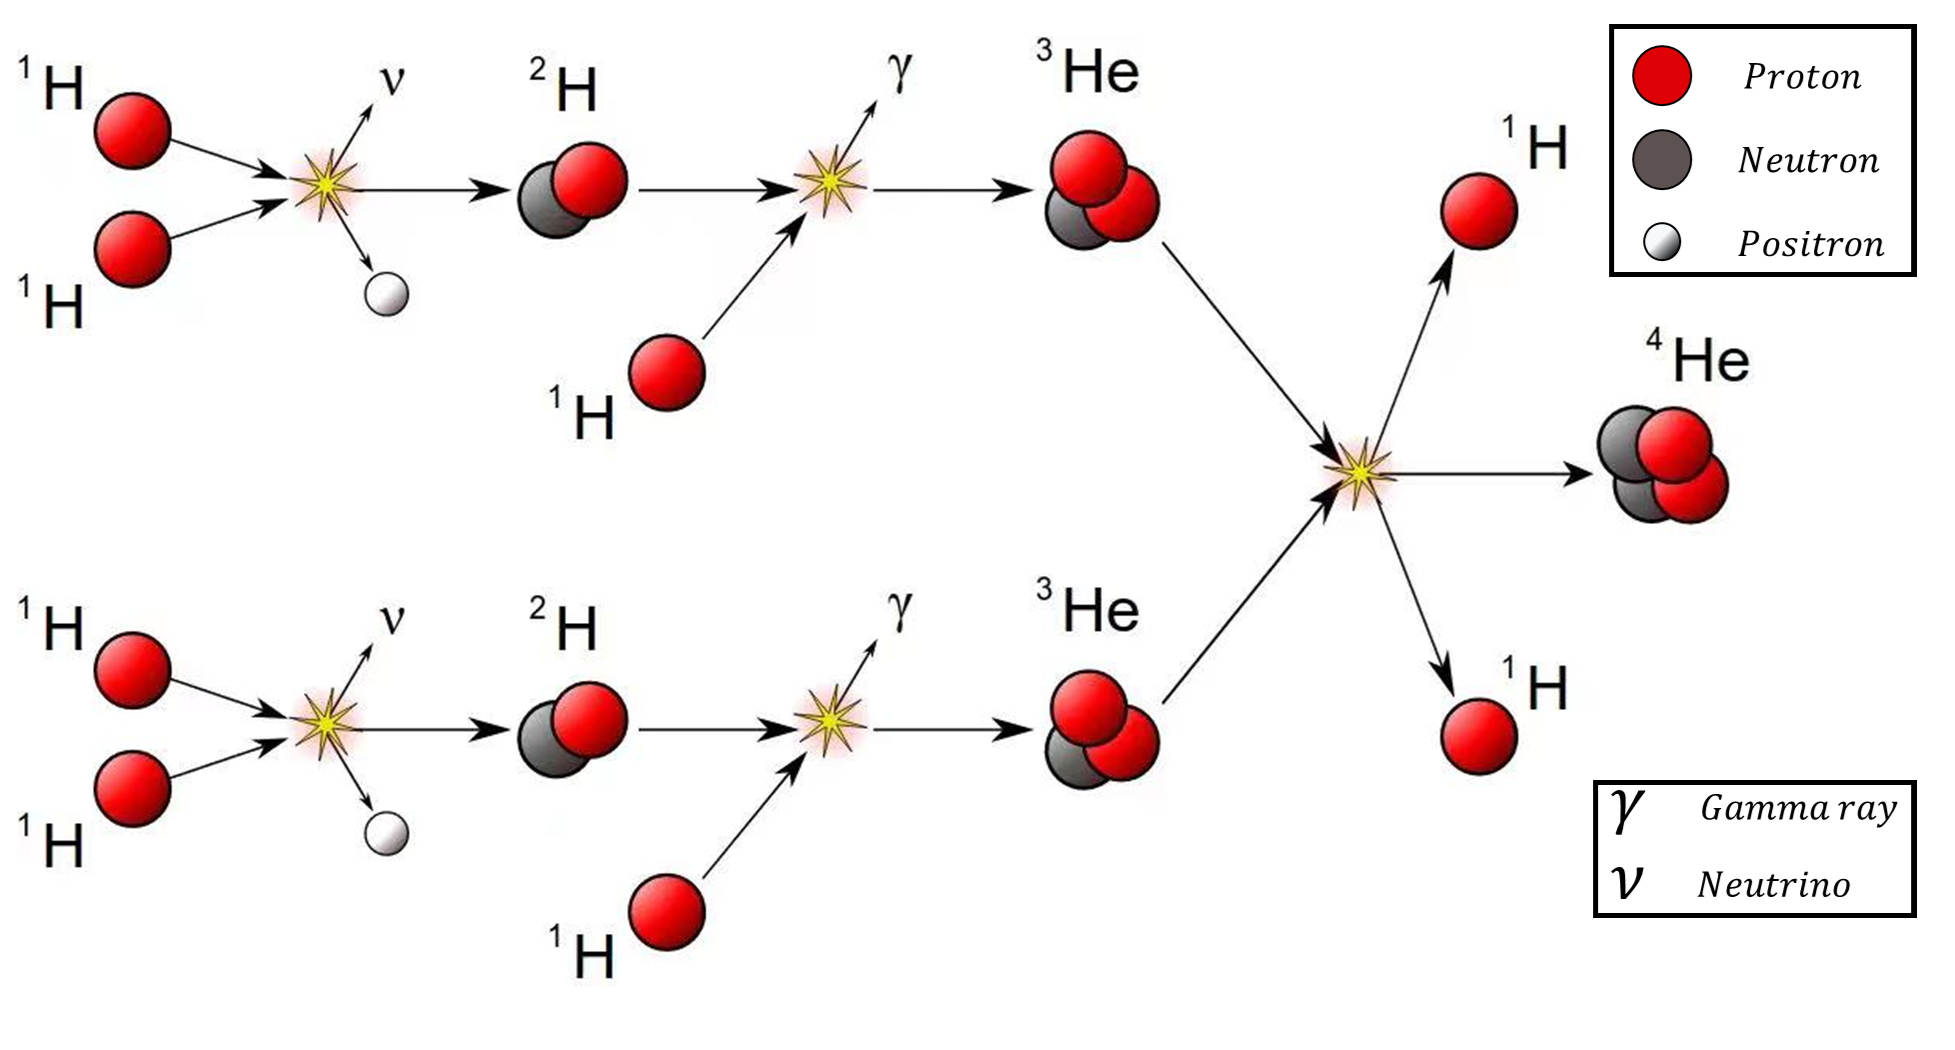
\includegraphics[width=14cm]{ppl_2.png}
\caption{\label{fig:ppI} p-p I 链式反应示意图,$^1H$代表质子,$^2H$代表氘核,$ν$代表电子中微子,
$^3He$代表氦-3 核,$^4He$代表氦-4 核,$γ$代表光子。反应朝箭头方向进行。\href{https://www.sun.org/encyclopedia/stars}{(https://www.sun.org/encyclopedia/stars)}
}
\end{figure}
\noindent     其中p代表质子,D代表氘核,e+代表正电子,$\nu_e$代表电子中微子,$^3He$代表氦-3核,$^4He$代表氦-4核,γ代表光子。反应按照箭头的方向进行。由于质子-质子衰变属于弱核力,反应效率很低,但是太阳的引力能长时间约束反应物,大量的反应物通过量子隧穿效应得以在太阳上能持续不断发生核聚变反应。然而地球上很难通过引力约束的方式产生受控核聚变,为了有效约束反应物,使之达到聚变反应条件,人们提出了惯性约束和磁约束等方式,其中磁约束中主流位型是托卡马克位型,如中国的EAST、美国的DIII-D以及未来的ITER。如\autoref{fig:tokamak}所示,托卡马克
\begin{figure}[ht]
\centering
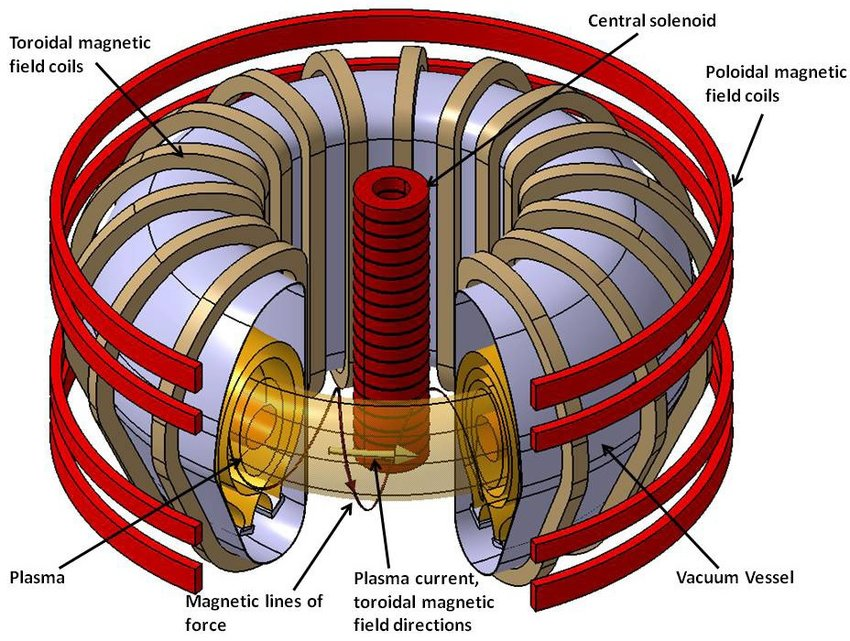
\includegraphics[width=12cm]{image2.jpeg}
\caption{\label{fig:tokamak} 托卡马克结构图\cite{RN950}}
\end{figure}
利用环向磁场和角向磁场将上亿度的等离子体约束在磁笼中,当密度、温度约束时间达到\href{https://www.energyencyclopedia.com/en/nuclear-fusion/thermonuclear-fusion/lawson-criterion}{劳森判据}时,即可实现自持的聚变燃烧。目前人们主要关注的聚变反应有$D-D$、$D-T$、$D-\text{He}^3$三种方式。\autoref{fig:D_D} 给出了它们的反应截面随温度的变化曲线,在温度较低时$D-T$反应相对于$D-D$和$D-\text{He}^3$具有更高的反应截面,高反应截面可以增加反应的概率和速率,从而提高反应效率,其相应的反应方程为:
\begin{equation*}
\begin{aligned}
&D+T\to\alpha(3.5\MeV)+n(14.1\MeV)\\
&D+D\to{}^3\text{He}(0.82\MeV)+n(2.45\MeV)\\
&D+{}^3\text{He}\to\alpha(3.6\MeV)+p^+(2.45\MeV)\\
\end{aligned}
\end{equation*}
海水中含有丰富的氘元素,根据氘氚反应方程可知3.8公升的海水可以产生相当于1135公升汽油的能量。面对未来的能源危机,受控核聚变为人类提供了一种绿色无限的能源。尽管有人称之为“永远的50年”,但能源的探索永不过时,因为我们的未来是星辰大海。
\begin{figure}[ht]
\centering
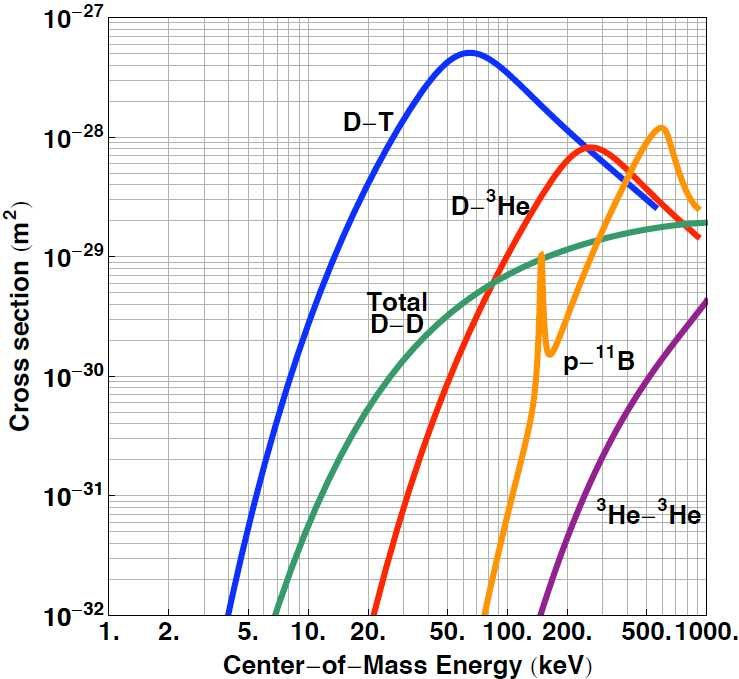
\includegraphics[width=12cm]{image3.jpeg}
\caption{\label{fig:D_D} $D-T$,$D-D$和$D-\text{He}^3$的反应截面,图片来自\cite{RN1698}}
\end{figure}
\clearpage
\section{托卡马克感应放电}
目前托卡马克放电主要通过中心螺线圈产生的感应电场实现对气体的电离并驱动带电粒子形成电流(如\autoref{fig:ohmdevice})。中心螺线圈感应放电一般分为三个阶段:电离或雪崩阶段、杂质烧蚀阶段和等离子体电流控制阶段\cite{RN2}。在托卡马克放电前中心螺线管预先储能,当放电指示下达时,中心螺线管通过电源和辅助电路的控制使电流开始下降,中心螺线管的磁通发生改变,在托卡马克环向会产生感应电场。关于该环电场强度的大小可以通过如下模型计算:中心螺线管外界电源电压为$V_{ps}$ ,外部电路的电阻为$R_{coil}$,电路电流为$I_{coil}$,根据电路基尔霍夫电压定律,中心螺线管的自感电压为$V_{coil}=V_{ps}-I_{coil}R_{coil}$,自感电压又可以表示为$V_{coil}=L_{coil}\frac{\dif I_{coil}}{\dif t}$,其中$L_{coil}$表示中心螺线管的自感系数,同时,考虑中心螺线管和等离子体之间的互感为M,绕大环方向一圈的环电压为$V_{loop}=M \frac{\dif I_{coil}}{\dif t}$,因此,$V_{loop}=MV_{coil}/L_{coil}$ ,在大半径为R处电场强度为$E=V_{loop}/2πR$。
\begin{figure}[ht]
\centering
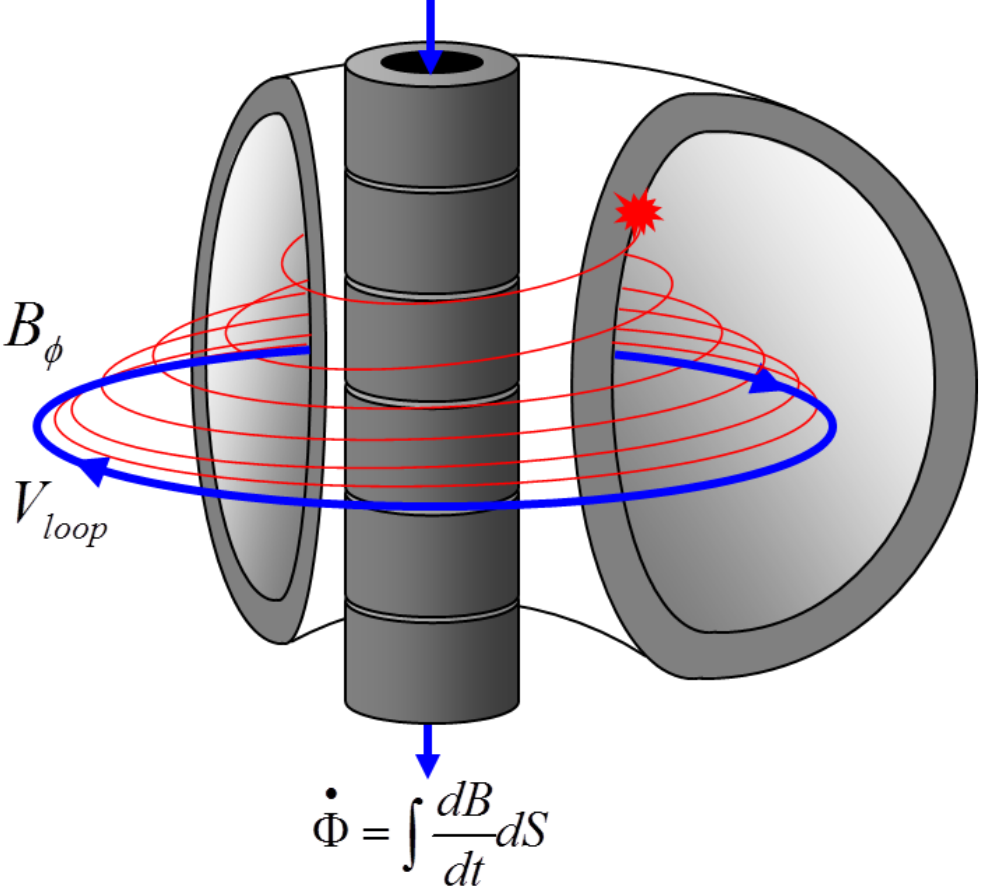
\includegraphics[width=12cm]{image4.png}
\caption{\label{fig:ohmdevice} 感应放电电子在环向磁场中的运动示意图\cite{RN951}}
\end{figure}
\par 托卡马克真空室中几乎一直存在自由电子,这些自由电子有可能来自于真空涨落,也有可能来自预电离的等离子体。放电启动时,这些自由电子在环电场作用下会被加速。当电子与下一个中性原子碰撞前动能超过$13.6\text{eV}$(氢原子的第一电离能,如果工作气体为氢气),电子就可能使中性原子电离并产生两个自由电子,新产生的电子会在环电场作用下继续加速,碰撞出更多的电子,这样的连锁反应过程称为汤森雪崩\cite{RN1234}。在雪崩过程中,单个电子单位路径产生α个自由电子,那么dx路径上就有d$n_e$=$αn_e $dx个电子产生,$n_e$表示电子密度,x表示沿电场方向的运动距离,积分得到具有指数增长的电子密度为$n_e=n_e (0) e^{αx}$,$α$表示第一汤森系数。击穿电离还涉及到击穿电场强度和预注入气体压强之间的关系,帕邢曲线描述了两板之间击穿电压和气压距离的关系,例如氦气的帕邢曲线如\autoref{fig:pxcurve}所示\cite{RN982},其中$V_b$表示电离击穿电压,d表示两板之间的距离,为了在最小的击穿电压下实现放电击穿必须对预填充气压做出合理的控制。托卡马克中电子绕中心
螺线管在大环方向上运动直到最后打在壁上所感受到的电压降V相当于帕邢曲线中的$V_b$,电子损失前运动的总路程称为连接长度L,类似于板间距d,如\autoref{fig:ohmdevice}红线所示。连接长度L与装置中的纵场$B_\phi$、杂
散场$B_s$ 以及小半径a有关,$L\sim a\cdot B_\phi/B_s $ ,例如在未来的ITER装置中,$B_\phi/B_s \sim10^{-3}$,$a=1-1.6m$,连接长度L约为1000m 。$\alpha/p$和$E/p$函数关系如\autoref{fig:pxcurve2} 所示\cite{RN1015}。 根据NSTX\cite{RN2}放电参数,$p\sim 5\times10^{-5}Torr$,$V_{loop}=2V/turn$,$α\sim10^{-2}/m$,电子在损失到真空壁前的约束路程必须要大于100m才能实现电子增益。托卡马克中电子在环向电场的驱动下主要沿环向磁场方向运动,但是由于磁力线弯曲、极向磁场、径向磁场梯度等因素,会使得电子在环向运动的同时还朝极向、径向运动,最终可能导致电子损失。为了在电子损失前有足够长的运动路程实现增益,在放电区域通常需要有零场区,这个位置只有环向磁场,极向磁场很小,电子在这个位置有足够长的连接长度,因此更容易电离击穿形成电流.
\begin{figure}[ht]
  \centering
  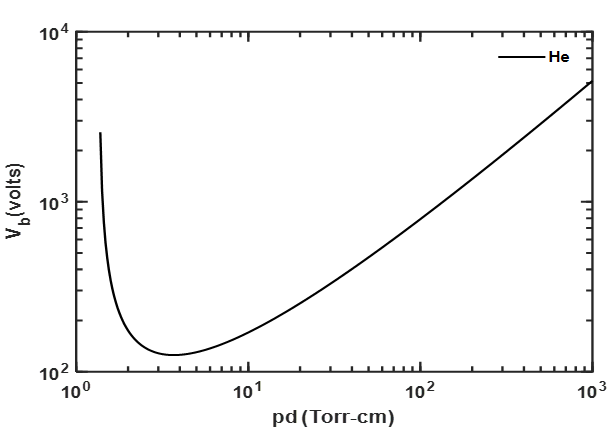
\includegraphics[width=12cm]{pxVb3.png}
  \caption{\label{fig:pxcurve} 氦气帕邢曲线图,pd表示气压×距离 }
\end{figure}


\begin{figure}[ht]
  \centering
  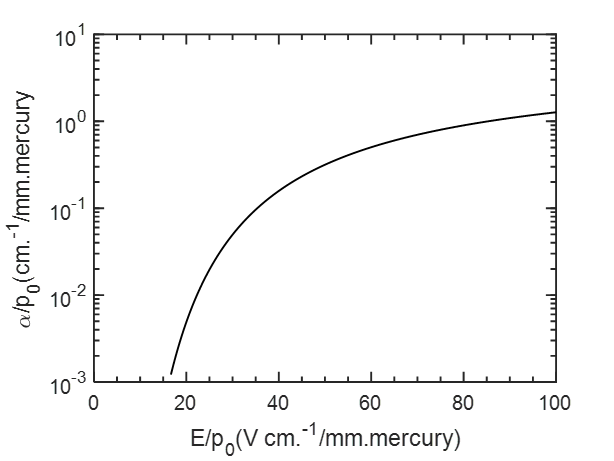
\includegraphics[width=12cm]{Ealpha2.png}
  \caption{\label{fig:pxcurve2} 电子在气体中单位路径产生的新电子数$\alpha$和电场E气压$p_0$的关系 }
\end{figure}

随着电离雪崩发生,中性气体的电离率越来越高,电子-电子的碰撞频率逐渐超过电子-中性气体的碰撞频率,当电离率超过$0.3\%$时,此时雪崩电离结束,进一步的电离过程是通过等离子体加热完成\cite{RN3}。在欧姆场加热等离子体过程中,除了电离消耗能量,杂质辐射会也会消耗能量,这些杂质主要来自壁材料如碳或铍氧,当杂质辐射能量和电离耗能超过欧姆注入的能量时,等离子体能量下降,电子重新和离子结合形成中性原子,最后导致放电失败。因此放电前通常会通过对内真空壁进行锂化处理、高温烘烤以及辉光放电清洗等手段降低壁中的碳氧等杂质,通过减少杂质或增加额外的注入功率,使放电继续维持下去。

杂质烧蚀过程中,等离子体电流也在爬升。当等离子体电流产生的极向磁场大于杂散场时,开放的磁力线将会闭合形成闭合磁面。电子绕螺旋闭合磁力线运动,其约束将会极大提升。当闭合磁面包含整个等离子体区域时电流产生的极向磁场将大于杂散场,即:
\begin{equation}
\frac{\mu_{o} I}{2 \pi a}>B_{s} \sim B_{\phi} \frac{a}{L} \rightarrow j=\frac{I}{\pi a^{2}}>B_{\phi} \frac{2}{\mu_{o} L}
\end{equation}
对于未来的ITER装置,杂散场$B_s=3mT$,连接长度L为1000m,纵场B为3T,小半径$a\sim1m$,等离子体电流$I$需要达到$15KA$才能形成放电区间完整的闭合磁面。\par
     磁面闭合后,在电流爬升中电子在环向场驱动过程下不断和周围的电子通过库伦散射交换能量,经过一定时间后大量电子开始呈现热分布的状态,此时等离子体具有了温度的概念。在纯欧姆放电条件下,等离子体通过欧姆加热机制提升温度。由于等离子体芯部约束高,一般情况下等离子体芯部温度上升更快,芯部电流也相对于更大。同向电流的pinch效应(洛伦兹力)使得等离子体有向内收缩的趋势,而压强梯度使得等离子体具有向外膨胀的趋势,二力平衡时等离子体达到稳定状态。还有一种情况也值得注意:由于欧姆加热效率与电阻率有关,温度越高电阻越低,随着等离子体芯部温度上升,芯部欧姆场加热效率也逐渐下降。携带电流的电子逐渐由热电子向非热化电子转移,而非热化电子主要为逃逸电子(关于逃逸电子在接下来的一小节会详细介绍)。由于逃逸电子碰撞阻尼小,该部分电子运动类似超导电子,类比伦敦第二方程可知逃逸电子会导致芯部感应电场下降,进而影响环向感应电场分布,改变环向电流分布。当满足一定条件时甚至会出现芯部电流低于边界电流的现象,也就是电流的趋肤效应。电流分布的空穴结构有可能导致撕裂模产生,破坏等离子体粒子约束\cite{duchs1972skin},也有可能会进一步提高等离子体的稳定性,促进聚变反应\cite{gourdain2009hollow}。因此放电初期对非热化电子的研究尤为重要。




%此时等离子体的平衡位型完全可由Grad-Shafranov方程描述,通过求解Grad-Shafranov方程获得的等离子体平衡位型为实验运行提供了重要参数。
    

\section{非热化电子产生机制}
	根据热力学定律,在没有外界影响下,一个热力学系统经过足够长时间后必然趋向于热分布,此时整个系统处于热平衡状态。对于托克马克中的电子,当电子速度分布通过碰撞散射达到热平衡分布时称为热电子,此时电子速度分布可以通过麦氏方程描述。但当电子速度分布偏离麦氏分布时称为非热化电子。导致电子速度偏离热分布的原因有很多,下面考虑欧姆场驱动下非热化电子的形成机制。\par
	通过试探粒子的方法可获得电子的等效阻尼力与电子动量的关系\cite{RN814,RN1817}(可参考附录\autoref{sec:A5})。如\autoref{fig:collisiondrag}中$F_c$所示,仅考虑库伦碰撞为电子加速过程中的等效阻力时,对于速度大于热速度的电子,库伦阻力与电子速度的平方成反比,当电子速度接近光速时受到的碰撞阻力达到最小值,如果电场力与这一最小碰撞阻力相当,则称该电场为Connor电场\cite{RN1875},凡是小于Connor电场的情况下均不可能存在逃逸电子,因此Connor电场也成为逃逸电子最小临界电场。当电场大于Conner电场时,碰撞阻尼小于电场力的电子将会受到加速,在加速过程中碰撞阻尼继续减小,最终电子将不断加速获得极高的能量, 因此该部分非热化电子称为逃逸电子。 然而实际情况下逃逸电场临界值通常大于Conner电场,这是因为存在磁场时,电子回旋辐射阻力会阻碍电子逃逸。如\autoref{fig:collisiondrag}中$F_{rad}$所示,电子回旋辐射阻尼$F_{rad}$随着电子速度增加而迅速上升,单电子其受到的总阻力为$F=F_{rad}+F_c$,这时电子的最小临界电场为$E_c^*$显然要高于$E_c$。当电场强度$E>E_c^*$时,处于动量区间$[p_1,p_2]$将发生逃逸,最终聚集在$p_2$点。在等离子体温度为$T_e$中电子的最大碰撞阻尼为热速度$v\approx v_{th}$所对应的平衡电场$E_s$,而与$E_s$同出一源的就是Dreicer电场
	\begin{equation}\label{eq:Dreicer_Field}
E_D=\frac{n_ee^3ln\Lambda}{4\pi \epsilon_0^2T_e}
\end{equation}
	Dreicer电场命名是为了纪念第一位研究等离子体中逃逸现象的科学家H.Dreicer\cite{RN954}。当电场强度达到$E_s\approx0.2E_D$时,整个等离子体中的电子都将发生逃逸,电子速度分布快速偏离麦氏分布,因此该电场称为side-away电场阈值。当电场只有百分之几的$E_D$,只有少量电子发生逃逸,刚刚逃逸出去的电子又会由于主体电子的扩散而得到补充,而主体电子的热分布特征并不会由于少量扩散而被改变,因此这部分少量的逃逸电子将会获得稳定的增长,这种逃逸电子的产生机制称为初级逃逸电子或Dreicer逃逸。
\begin{figure}[ht]
  \centering
  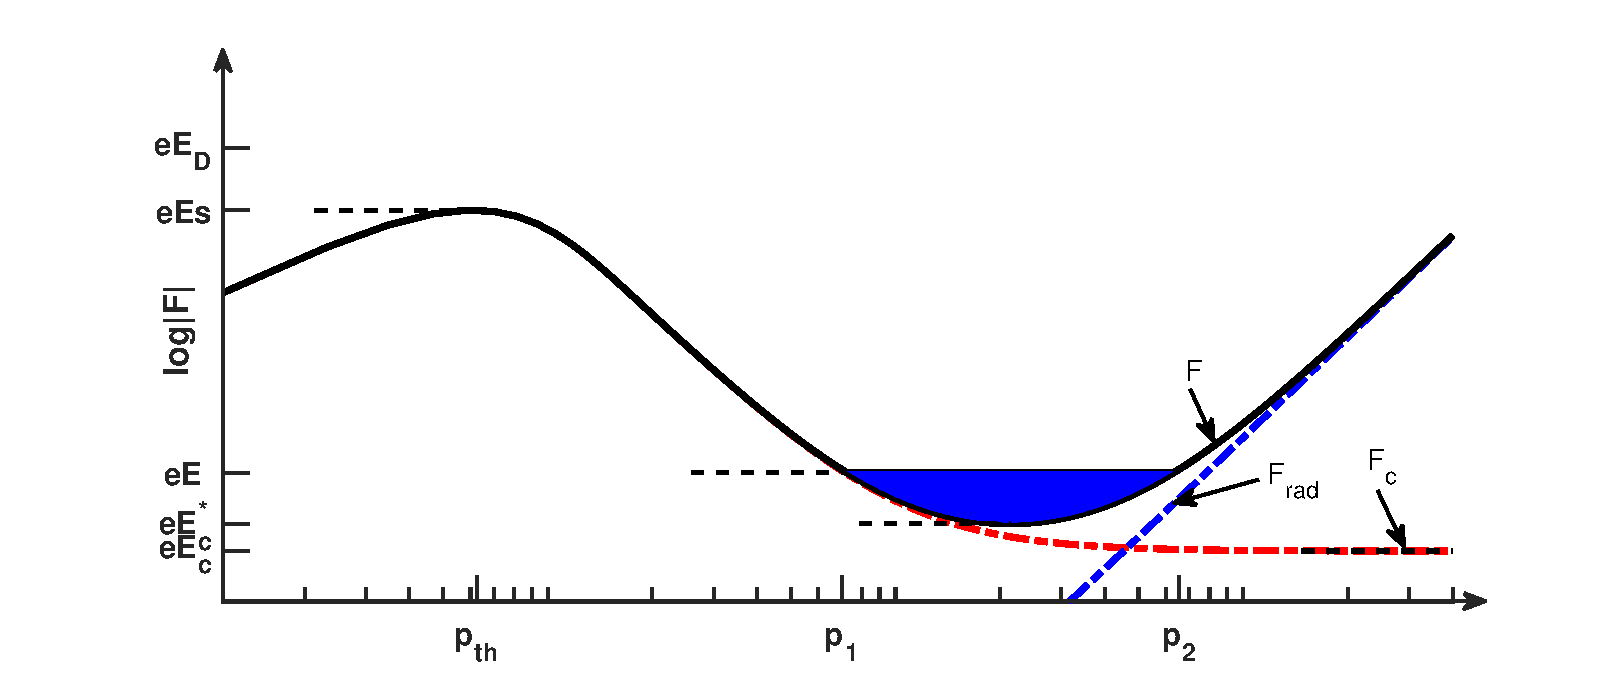
\includegraphics[width=16cm]{image7.eps}
  \caption{\label{fig:collisiondrag} 库伦碰撞阻力$F_c$、辐射阻力$F_{rad}$以及合力$F$随动量分布 }
\end{figure} 
\par
除了以上讨论的电场驱动电子逃逸过程,逃逸电子的另一种产生机制是通过大角度碰撞,也称为雪崩机制\cite{RN1793}。这种机制可以简单如下描述:一个具有高能量的逃逸电子和热电子发生大角度碰撞,碰撞后的两个电子速度均超过了临界速度然后形成两个逃逸电子,然后一生二,二生四,逃逸电子的数量就以雪崩指数增长。当然不是所有逃逸电子都能发生雪崩机制,在等离子体中由于辐射效应以及各种不稳定性限制导致逃逸电子存在能量上限\cite{RN874}。当系统中具有最大能量的电子和热电子碰撞后仍然不足以使碰撞后的两个电子都大于逃逸的速度,雪崩效应就不会发生。只有当电场大于一定值,逃逸电子能量足以产生逃逸电子对,雪崩效应才会产生。Aleynikov通过近似理论计算了有效电荷数Z为5,密度为$10^{20}~m^{-3}$,温度为$1~KeV$,磁场为$1.81~T$雪崩电场阈值$E_a$约为$1.8E_c$。然而后来基于玻尔兹曼碰撞算符数值模拟到的结果却表明不存在雪崩电场阈值\cite{RN1811},该部分内容会在\autoref{sec:no_growth}讨论密度下降过程回旋辐射问题时有详细讨论。

综上所述逃逸电子的产生存在两个临界电场:$E_c^*$表示产生逃逸电子所需最低电场;$E_s$表示所有电子均发生逃逸的临界电场,此时放电称为side-away放电。由于逃逸电子的能量上可达几十MeV,当其轰击到装置内壁时会对装置造成严重破坏,因此在放电过程中对逃逸电子的控制格外重要。如果能通过某种机制把平行磁场方向的电子动能转换到垂直方向,增大辐射阻尼的同时也增大了电子运动轨道长度,进而抑制逃逸电子的产生,对保护装置\cite{RN1866}和实现聚变均有所裨益。我们将在论文的\autoref{sec:simulationVPA}对这一机制进行详细讨论。

辅助加热也是非热化电子产生的重要途径。如低杂波加热过程中,电子速度和低杂波相速度满足共振条件时电子就会通过朗道阻尼获得能量成为非热化电子。 如\autoref{fig:nonths}所示,非热化电子会对电流分布产生影响,驱动MHD不稳定性,MHD不稳定性产生的磁扰动又会感应新的电场进一步影响非热化电子的产生。这种种关系或正反馈或负反馈构成了复杂多变的等离子体环境。托卡马克许多物理过程中都与非热化电子密切相关,如ELM\cite{RN1868}、Sawtooth\cite{RN1917}、Disruption\cite{RN985}等过程中都会产生非热化电子,而非热化电子对等离子体反常输运\cite{RN986}、误差场的穿透不稳定性\cite{RN987}、等离子体的加热过程\cite{RN1697}也有重要影响。

在纯感应放电过程中,逃逸电子的形成过程可以解释电子为什么会在平行磁场方向上产生MeV的动能,但无法解释实验中非热化电子垂直方向能量为什么可以达到百keV\cite{RN726}。首先可以排除是欧姆加热机制,因为热电子的温度通常只有keV,温度越高电子库伦碰撞频率越低,无法通过库伦碰撞产生百keV的能量。在垂直磁场方向具有百keV能量的非热化电子是如何产生的?关于这个问题目前有以下解释:
\begin{itemize}
\item 无碰撞散射过程\cite{RN1794} \par
由于托卡马克中磁场具有螺旋结构,电子在运动过程中感受到的磁场环境是不断变化的,导致电子的磁矩不再守恒,平行磁场方向加速的电子被背景磁场散射导致垂直磁场方向动能增大。
\item 电子雪崩过程\cite{RN1793} \par
背景电子被逃逸电子碰撞产生的大角度散射也是导致电子垂直方向能量升高的原因。
\item 反常多普勒效应(ADE,Anomalous Doppler Effect)\par
反常多普勒效应是电子和波相互作用产生的一种不稳定性。笼统地解释是在电场的驱动下,逃逸电子的能量逐渐增大,当能量达到一定阈值时,满足$ω-\vk\cdot \vv+nω_{ce}=0$\cite{RN1757}共振条件的波就会被激发出来。当n>0时对应反常多普勒共振,被激发出的波又会反过来作用于逃逸电子导致电子平行磁场方向的能量迅速转移到垂直磁场方向上,这样逃逸电子在垂直磁场方向的能量就会快速增加,这里ω表示激发出的波,$k_z$表示沿磁场方向的波矢,$v_z$表示电子平行磁场方向的速度,$ω_{ce}$表示电子回旋频率,n表示共振阶数。
\end{itemize}

\begin{figure}[ht]
  \centering
  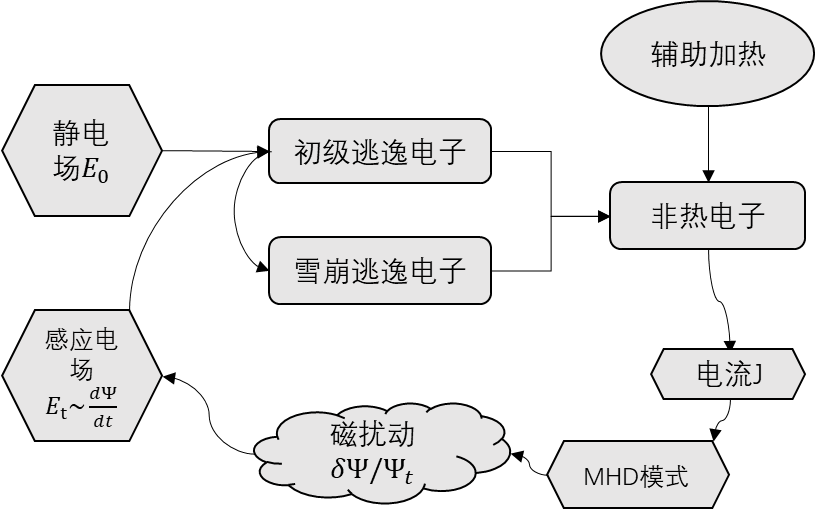
\includegraphics[width=12cm]{image8.png}
  \caption{\label{fig:nonths} 非热电子产生途径示意图 }
\end{figure}
那么ADE为什么会导致电子动量的快速散射?其物理机制是什么?关于这些问题目前的分析大都是建立在准线性理论分析上\cite{RN1801},从速度分布函数的演化角度解释散射,但ADE的物理本质并没有得到很好的理解,本文将在\autoref{sec:ewmele}对ADE效应的物理本质展开研究。
\par ADE机制与其它两种机制的最大区别就是存在一个由非热电子本身驱动的波。在托卡马克实验中已经有很多与ADE机制相吻合的实验观测\cite{RN975,RN798,RN786,RN1868},其中最明显莫过于放电初期的电子回旋辐射,我们将在第二章具体展开讨论。

\section{反常多普勒效应}\label{sec:quantum}
ADE是电子和波相互作用产生的一种不稳定性\cite{RN782},当电子在磁场中运动时,这种不稳定性会导致电子平行磁场方向的能量迅速散射到垂直磁场方向上。ADE效应最早是Ginzburg\cite{RN1352}, Tamm\cite{RN2008}以及I.M.Frank\cite{RN2009}提出的理论猜想,并且Tamm和I.M.Frank在1958年诺贝尔获奖报告上详细介绍了ADE理论。现在简单介绍这一不同寻常的现象:\par
如\autoref{fig:cherenkov}所示,当带电粒子以超过介质中光速的速度穿过介质时,将在介质内产生诱导电流。这些诱导电流会激发次波,并与运动粒子的电磁场相互干涉,从而产生切伦科夫辐射(Cerenkov Radiation\cite{RN1861})。此时辐射波矢k的传播方向只能沿着切伦科夫辐射角$cos(θ_0)=c/(vn(\omega))=\frac{c'}{v}=\frac{\omega}{kv}$。现在我们考虑把自由带电粒子替换成具有内能和动能的系统(如一个运动的振子或一个沿磁力线运动的回旋电子等)。如\autoref{fig:radreg}所示,该系统在折射率为$n(\omega)$的空间中超光速运动($v>c/n(ω) $)并辐射出具有角频率为$ω$的光子(图中$θ$表示光子辐射方向$\vk$和运动方向$\vv$的夹角),此时光子的方向可以沿任意方向,不依赖于次波叠加干涉。根据能量守恒和动量守恒关系,我们有
\begin{figure}[ht]
\centering
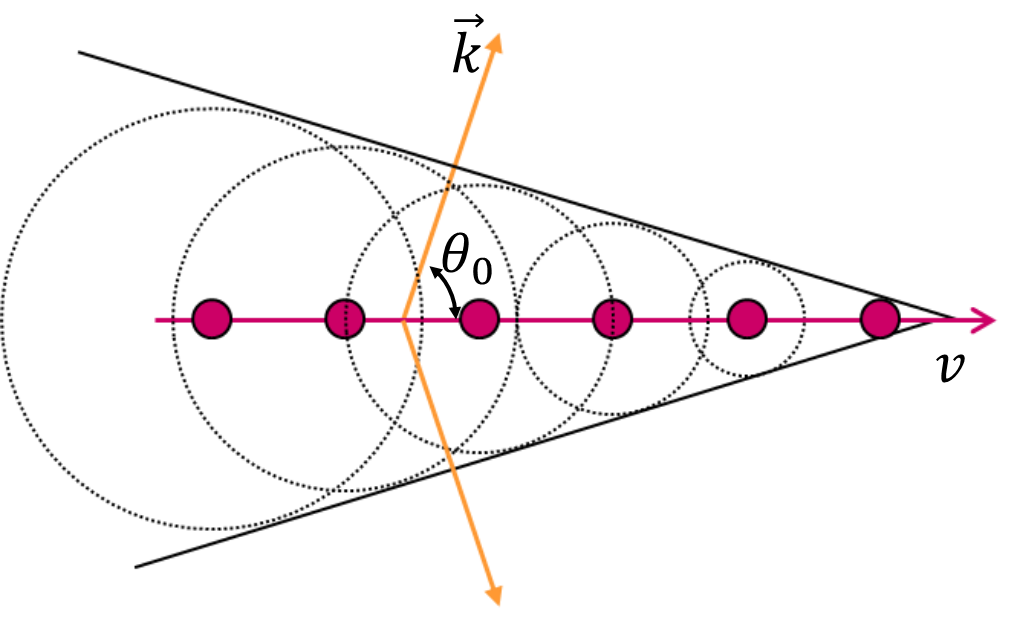
\includegraphics[width=12cm]{cherenkov.png}
\caption{\label{fig:cherenkov}实验室坐标系下粒子速度为$v$时切伦科夫辐射图\href{http://large.stanford.edu/courses/2014/ph241/alaeian2/}{(http://large.stanford.edu/courses/2014/ph241/alaeian2/)}		}
\end{figure}
\begin{figure}
\centering
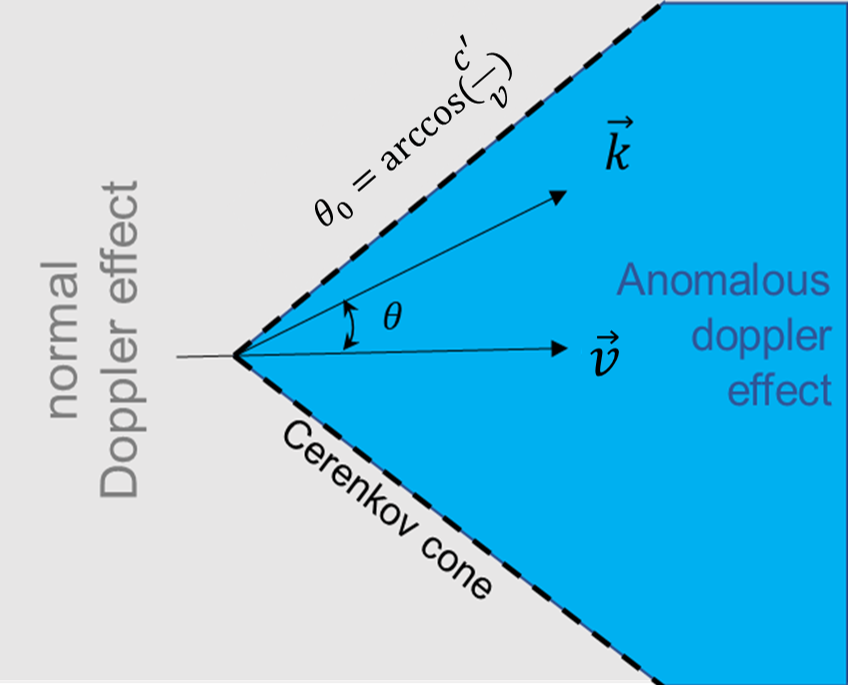
\includegraphics[width=12cm]{image21.png}
\caption{\label{fig:radreg}实验室坐标系下不同类型辐射区间分布,图片改自(X.H.Shi\&X.Lin)\cite{shi2018superlight}}
\end{figure}
\begin{equation}\label{eq:UT}
\begin{aligned}
T_1+U_1&=\hbar \omega+T_2+U_2 \\
\vp_1&=\vp_2+\hbar \vk 
\end{aligned}
\end{equation}

其中$T_1$和$U_1$表示系统初始具有的动能和内能,$T_2$和$U_2$表示辐射出光子后系统具有的动能和内能。考虑到光子能量远远小于系统具有的动能,$ℏω\ll T_1$,系统损失的动能可表示为$ΔT_{12}=T_1-T_2=Δ\vp\cdot\vv$,其中$\vv$表示辐射光子前系统的运动速度,$Δ\vp=\vp_1-\vp_2=\hbar\vk$。根据\autoref{eq:UT},我们有
\begin{equation}
\begin{aligned}
\Delta U_{21}=&ΔT_{12}-\hbar\omega\\
=&\hbar \vk \cdot \vv-\hbar \omega \\ 
=&\hbar \omega\left(\frac{k v \cos \theta}{\omega}-1\right)
\end{aligned}
\end{equation}
这里$ω/k=c/n(ω)=c'$ ,$\Delta U_{21}=U_2-U_1$。从方程中我们可以得到三点重要信息:\\
1.当$θ<θ_0 ,ΔU_{21}>0$,系统损失的动能转化为光子能量和系统的内能;\\
2.当$θ=θ_0,ΔU_{21}=0$,系统损失的动能完全转化为光子能量;\\
3.当$θ>θ_0,ΔU_{21}<0$, 系统通过消耗自身的内能和动能产生光子。\\

根据$ΔU_{21}$的正负,我们把辐射分为三种效应,其中$ΔU_{21}<0$称之为多普勒效应(NDE,Normal Doppler Effect),多普勒效应会消耗自身的内能和动能;$ΔU_{21}>0$为反常多普勒效应;$ΔU_{21}=0$称之为切伦科夫效应。当系统速度超光速$(v>c/n)$时,这三种效应均有可能产生,而当系统速度小于光速时$(v<c/n)$,只存在多普勒效应。
   \par 现在我们考虑这样一个特殊的系统:均匀磁场背景下平行于磁场方向运动的回旋电子。在该系统中,沿磁场方向电子以速度$v$自由运动,电子在垂直磁场方向上具有微小的速度$v_⊥$,假设在背景磁场强度为$B$的电子回旋能量(相当于内能)改变量满足量子化 \cite{RN1969}
\begin{equation}
\Delta U_{21} = n \hbar \omega_{ce},\omega_{ce}= \frac{eB}{m_e}
\end{equation}
这里$m_e$表示电子质量,$n=0,±1,±2,……$根据能量守恒定律,我们有:
\begin{equation}\label{eq:quantum energy}
ℏ\vk \cdot \vv=ℏω+nℏω_{ce}
\end{equation}
或
\begin{equation}
ω-\vk\cdot\vv=-nω_{ce}
\end{equation}
其中$ℏ\vk \cdot \vv$表示损失的动能,$ℏω$表示产生光子的能量,$nℏω_{ce}$表示电子回旋内能增加量($\Delta U_{21}$),$n$为整数。\autoref{eq:quantum energy}所包含的物理是:损失的动能$ℏ\vk \cdot \vv$转化为系统的内能$nℏω_{ce}$和光子能量$ℏω$。当$n<0$时对应多普勒效应,电子辐射光子后动能和回旋内能均降低;当$n=0$时对应切伦科夫效应,辐射的光子不会导致电子回旋内能任何改变;当$n>0$时对应ADE,根据能量方程$ℏ\vk\cdot\vv=ℏω+nℏω_{ce}$,电子平行方向动能的变化量转化为光子能量和增加的回旋内能。以上通过量子效应解释了ADE效应的能量转移特征,也可以从经典力学角度来考虑ADE的物理过程,我们将在论文\autoref{sec:ewmele}介绍磁化电子和电磁波相互作用时对ADE效应的力学机制进一步探究。根据ADE效应,如果在辐射光子前电子没有回旋内能只有平行方向的动能,那么在辐射光子后电子平行磁场方向动能将会向垂直方向转移。例如在电子束流实验中,ADE会使电子束流单一的速度方向发生弥散,这些现象已经被实验验证\cite{RN798,RN1862}。
\begin{figure}[ht]
\centering
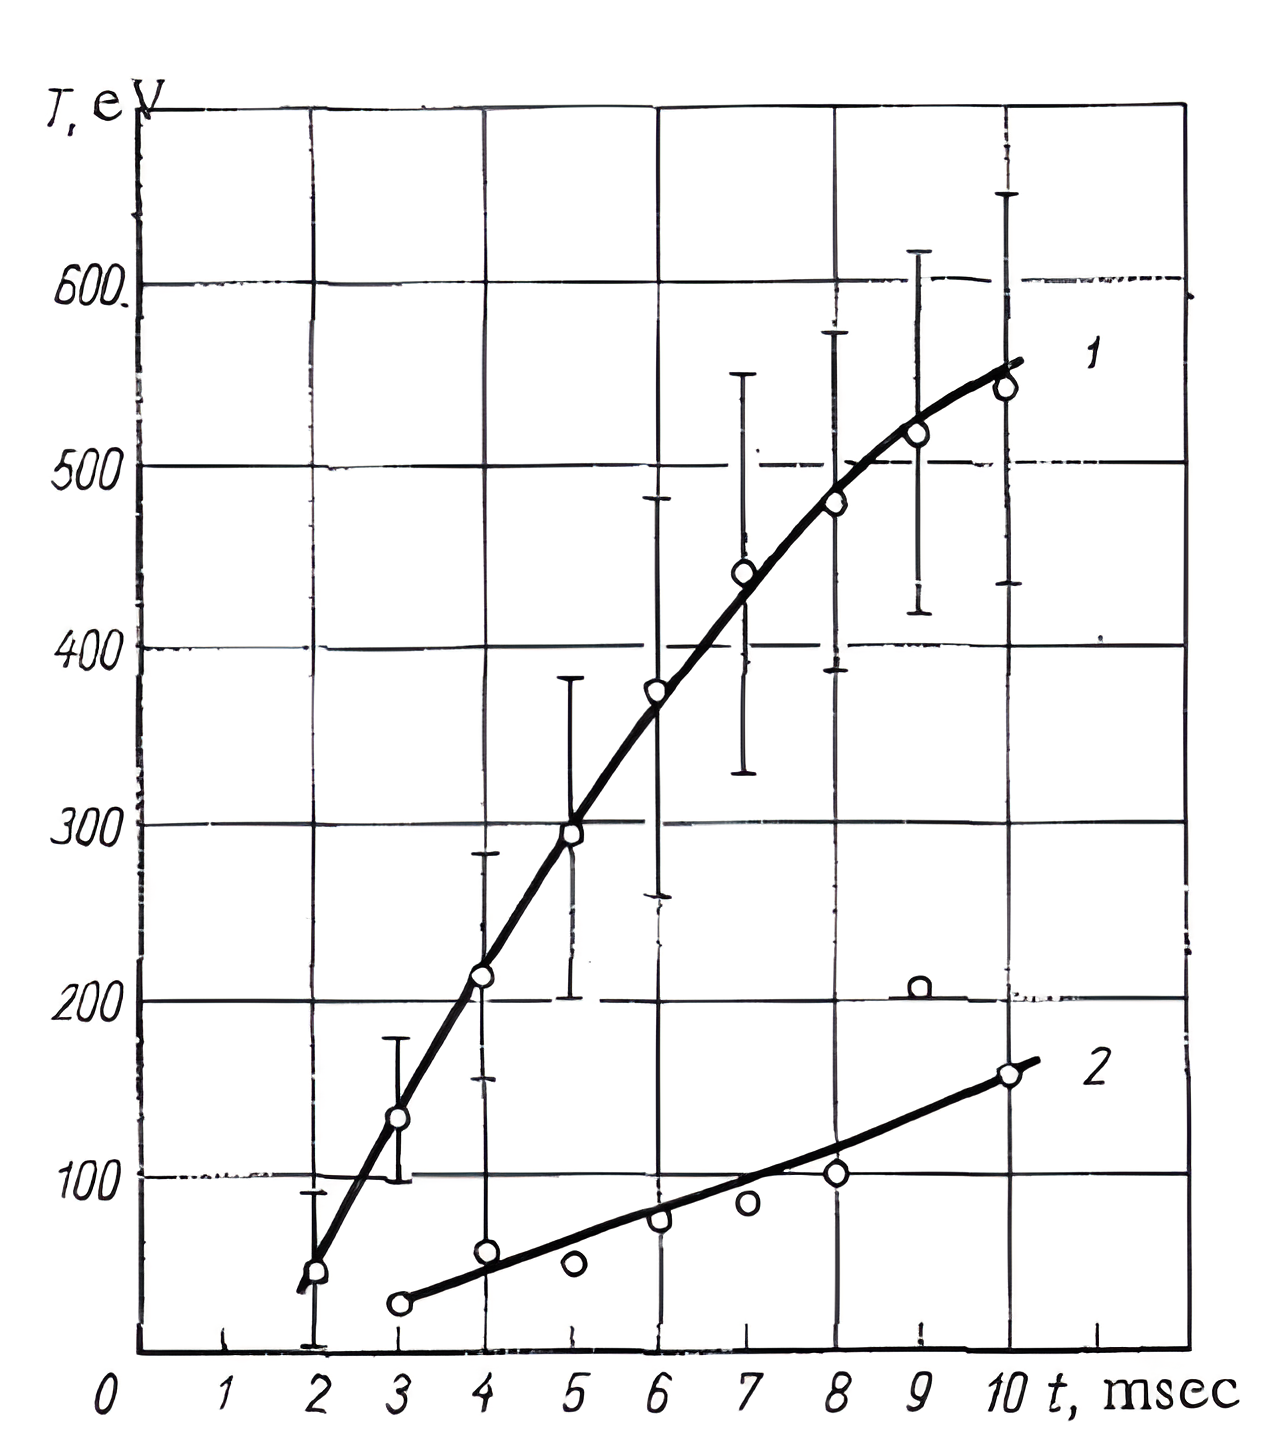
\includegraphics[width=10cm]{image22_1.png}
\caption{\label{fig:LAA}曲线1:抗磁性效应测量的$T_e + T_i$;曲线2:通过电导率测量的电子温度$T_{eσ}$}
\end{figure}
\par
1967年,前苏联L. A. Artimovich在 T-3托卡马克装置和TM-3托卡马克装置中分别用逆磁效应和经典等离子体电导率测量等离子体温度\cite{RN1863}。逆磁效应是磁化等离子体中常见的现象,其原因是因为电子和离子自旋产生的磁场方向和背景磁场相反,当电子或离子温度越高,逆磁效应越加显著,因此
可以通过测量托卡马克环向磁通的变化量反推出等离子体温度,同时通过测量环电压和等离子体电流可算出等离子体平均电导率,根据经典电导率和温度之间的关系同样可以推导出等离子体温度。如\autoref{fig:LAA}实验发现,通过逆磁效应测出的温度远大于等离子体电导率测出的温度 ,反过来说通过逆磁温度推导出来的电导率远大于实验测得的电导率,由于缺少合理的物理解释,对这种低于经典电导率的实验现象当时称为反常电导率。

\par 1968, B. B. KADOMTSEV指出L. A. Artimovich测到的反常电导率是由于ADE造成\cite{RN964},由于沿平行磁场方向运动的电子在ADE作用下电子向垂直磁场方向散射,导致逆磁效应增加,使得根据逆磁效应得到的电导率高于真实电导率。同年V. D. SHAPIRO\cite{RN1425}提出了等离子体中反常多普勒过程的准线性理论,等离子体中ADE开始逐渐引起人们重视。
\par 1971年E. G. SHUSTIN利用微波天线和静电场能量分析器研究磁场背景下真空放电管等离子体束不稳定性\cite{RN786},如\autoref{fig:EGS1}所示,\autoref{fig:EGS1}上图是整个系统框架,包括真空放电管,可移动微波探
\begin{figure}[ht]
\centering
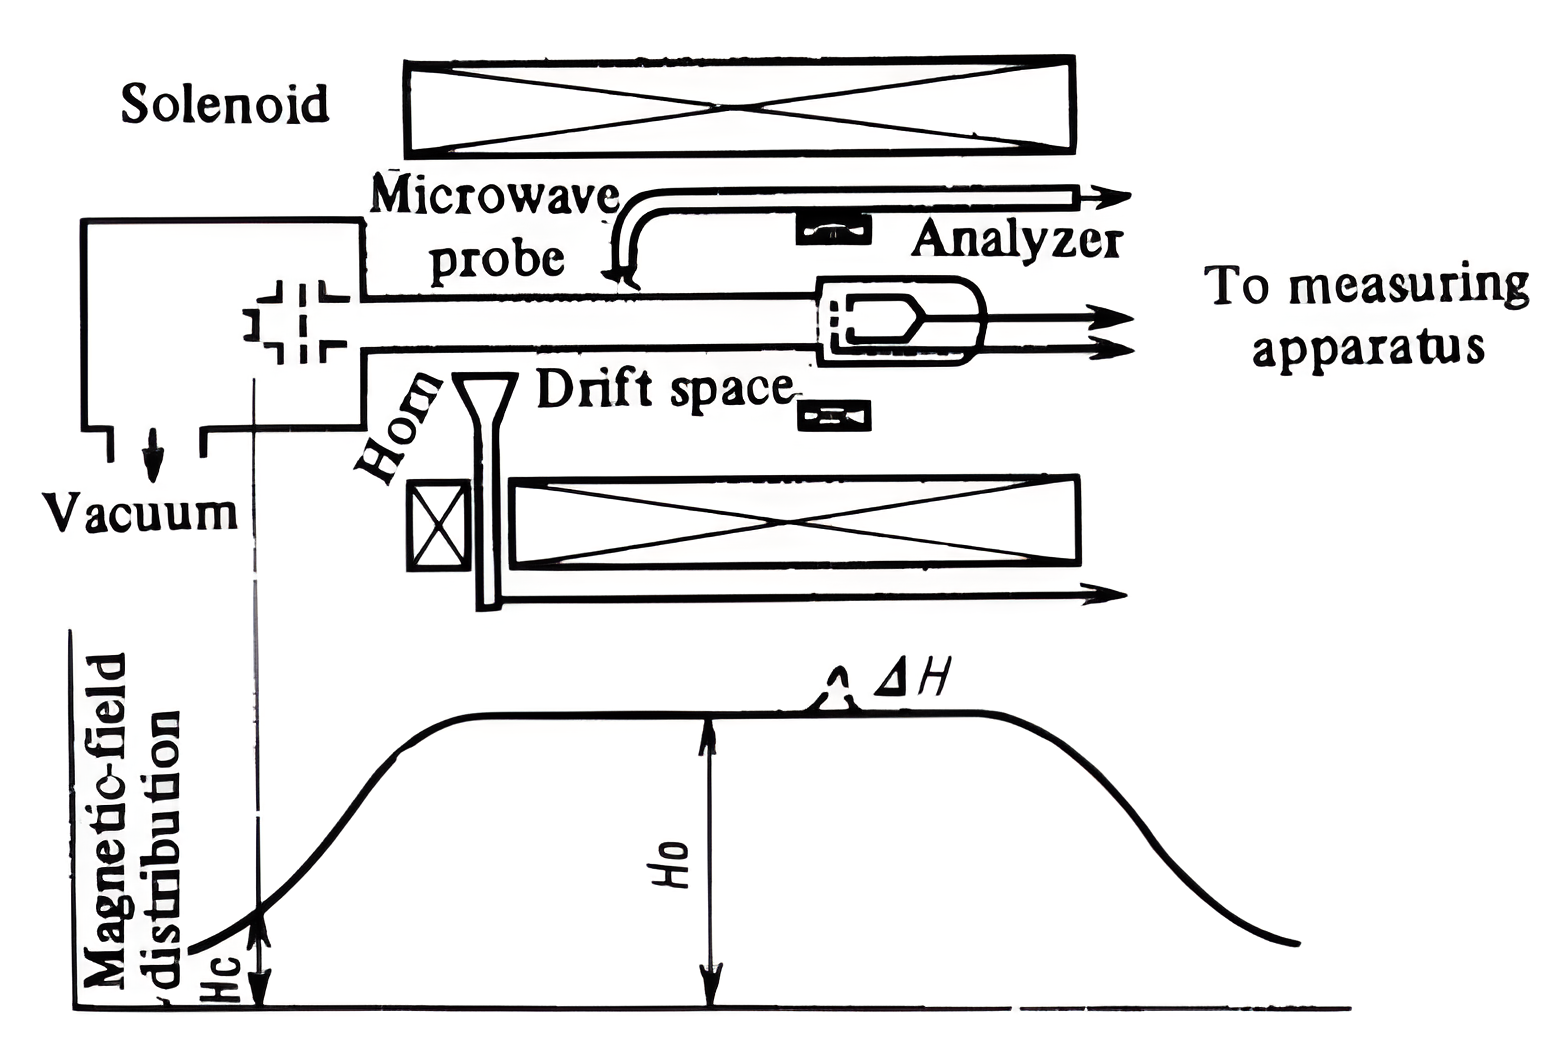
\includegraphics[width=12cm]{image23_1.png}
\caption{\label{fig:EGS1}实验设置}
\end{figure}
针,轴向场线圈以及静电场能量分析仪,静电场能量分析仪由偏压为$U_r$的栅网和用于产生磁镜的线圈构成。\autoref{fig:EGS1}下图表示真空放电管中由轴向场线圈和磁镜线圈构成的总磁场强度分布。静电场能量分析可用于获得束等离子体轴向速度分布函数和轴向速度在$v_∥$和$v_∥+dv_∥$区间具有的横向平均能量。根据不同的$h=ΔH/H_0 $曲线可以测得电子轴向速度$v_∥$对应的横向运动的平均能量为
\begin{equation}
\bar{W}_{\perp}\left(v_{\|}\right)=\frac{\int W_{\perp} f\left(v_{\|}, v_{\perp}\right) d v_{\perp}}{\int f\left(v_{\|}, v_{\perp}\right) d v_{\perp}}=\left.\frac{\frac{\partial I}{\partial h}}{\frac{\partial I}{\partial U_{r}}}\right|_{h \rightarrow 0}
\end{equation}
其中I 表示延迟电流。

实验结果表明,当放电真空管保持良好的真空条件时$(p=10^{-6}mm Hg)$时,电子束分布基本保持在初始速度$v_0$附近,如\autoref{fig:EGS2}(后图)所示,垂直能量基本不超过60eV,极小部分由于磁场不均匀性导致垂直能量达到300eV。当放电真空管残余气体压强增加时,管中等离子体产生双流不稳定性,此时会激发出$\omega< \omega_p$的纵波,从结果来看,这种纵波最终会导致分布函数拉平(\autoref{fig:EGS2}中间),束电子横向最大能量进一步升高到450eV,而拉平分布函数的极有可能是朗道阻尼机制。当放电真空管残余气体压强继续增加到$2.1\times10^{-3}mm Hg$(\autoref{fig:EGS2}前图),电子平行磁场方向能量跳跃式散射到垂直磁场方向,伴随着处在电子回旋频率$ω_{ce}$和等离子体上杂化频率$\sqrt{ω_p^2+ω_{ce}^2}$区间的微波信号产生,且微波极化方向垂直于轴向磁场方向。最终横向能量最大增加到$1500eV$,大部分横向能量达到$500eV$,该现象为反常多普勒效应提供了直接实验证据。
\begin{figure}[ht]
\centering
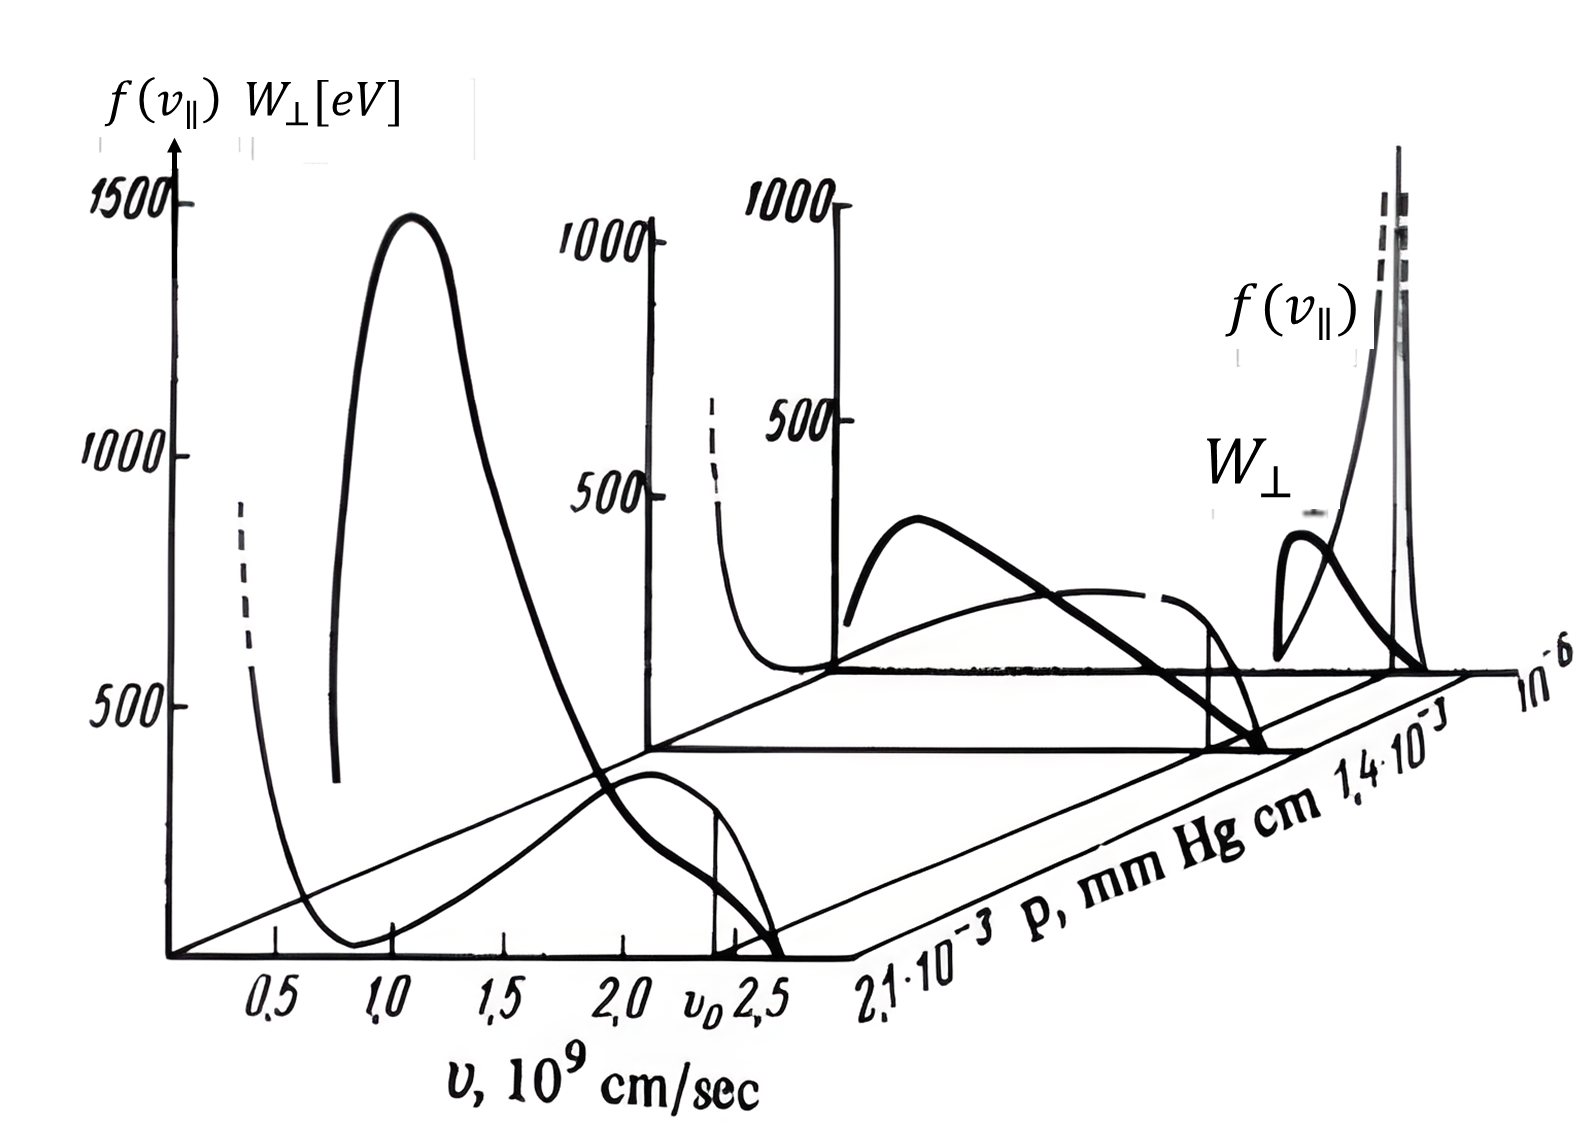
\includegraphics[width=12cm]{image24_1.png}
\caption{\label{fig:EGS2}轴向速度分布函数$f(v_{||})$(细线)和横向平均能量$W_⊥$(粗线);$v_0$表示束电子初始速度\cite{RN786}}
\end{figure}
\par
1976年D.A.Boyd在ATC首次发现电子回旋辐射step结构\cite{RN725},1979年,H. Knoepfel将D.A.Boyd观测到的step现象归因于反常多普勒效应\cite{RN1030}。
\par
1984年,F. Santini在Frascati 托卡马克装置低密度放电条件下,验证了低杂波通过反常多普勒效应对逃逸电子能量的影响\cite{RN1866},实验中逃逸电子能量分别通过硬X射线(H-Xray)和光核反应中子探测,其中硬X射线来源于逃逸电子打在限制器上产生的轫致辐射,电子能量只需要大于500keV就能被有效探测,光核反应中子探测用于探测更高能的电子(14MeV-25MeV)和高z材料相互作用产生的高能$γ$射线和原子核相互作用诱导原子核放出中子,其中等离子体中D-D反应和e-D反应产生的中子可作为背景辐射忽略不计。如\autoref{fig:FST}所示
\begin{figure}[ht]
\centering
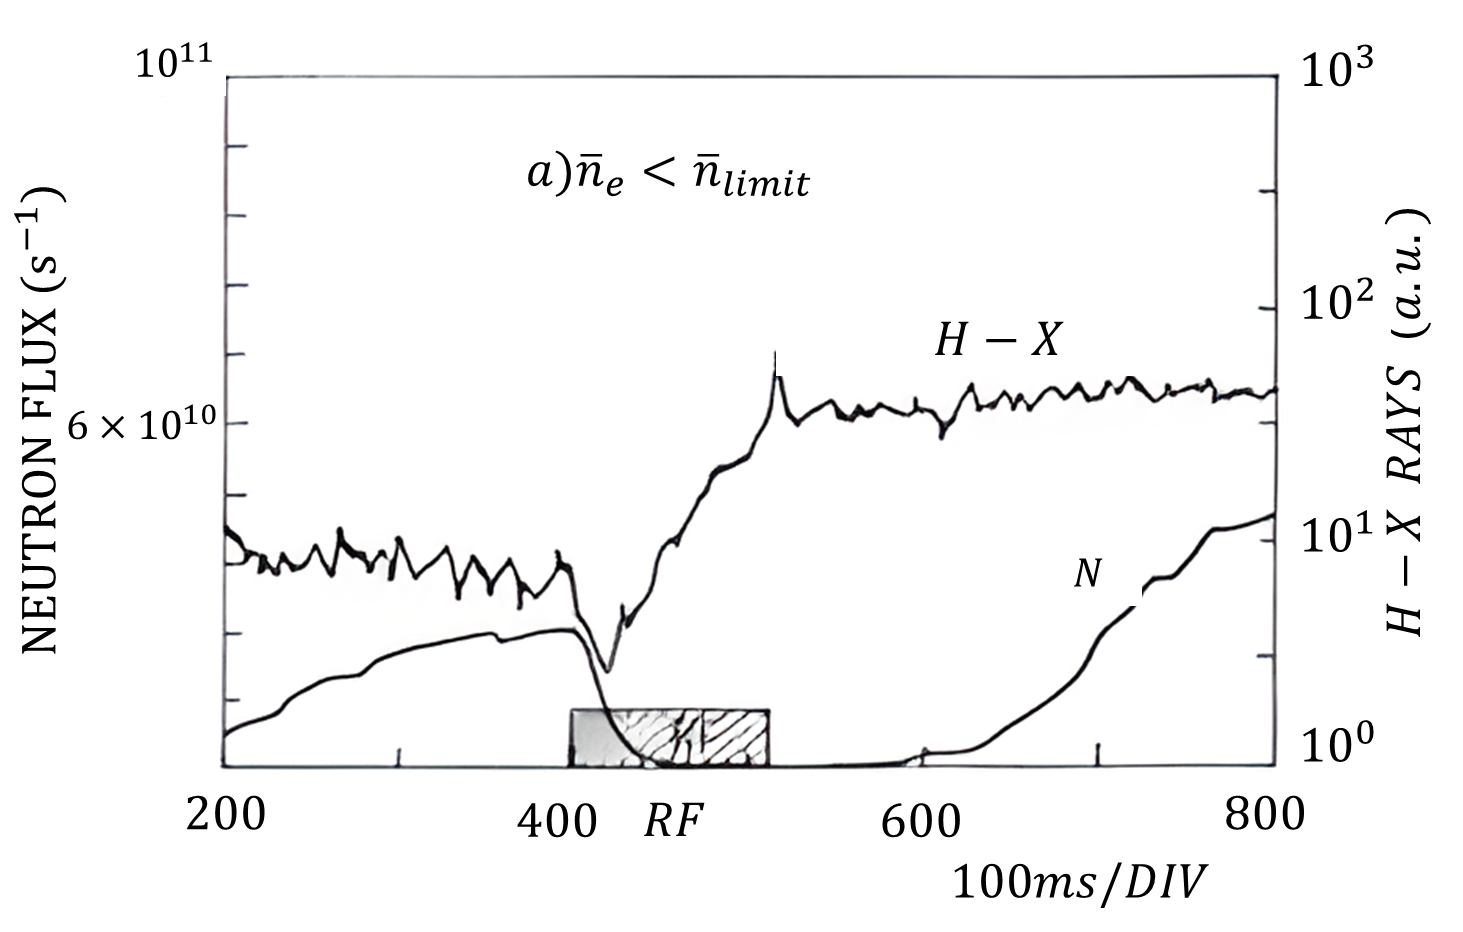
\includegraphics[width=12cm]{image26_1.png}
\caption{\label{fig:FST}氢放电过程光核反应产生的中子和H-X射线的时间演化行为\cite{RN1866}}
\end{figure}
,H-X表示硬X射线,N表示中子辐射,RF表示低杂波注入,从图中可以看出,当RF注入开始时,H-X强度和中子辐射同时开始下降,随后H-X和中子辐射又逐渐上升,这一现象可以通过反常多普勒共振理论和朗道共振解释:当低杂波注入时,高于15MeV高能电子由于和低杂波满足反常多普勒共振条件,高能电子能量向垂直磁场方向散射,逃逸电子动能下降,H-X和中子辐射降低。在低密度条件下,低杂波和电子通过朗道共振使电子速度分布函数形成高达300keV高能尾巴,而逃逸电子临界能量远低于300keV,因此这些电子在环电场驱动下逐渐形成高能逃逸电子,最后导致HX和中子辐射再次上升。

2009年,陈忠勇等人在HT-7托卡马克装置上研究了\autoref{fig:CZY1}step结构产生阈值$ω_{pe}/ω_{ce} $和磁场电流的关系。如\autoref{fig:CZY2}所示,实验结果表明step结构产生阈值和电流存在线性依赖关系,和磁场无关\cite{RN1554}。
\begin{figure}[ht]
\centering
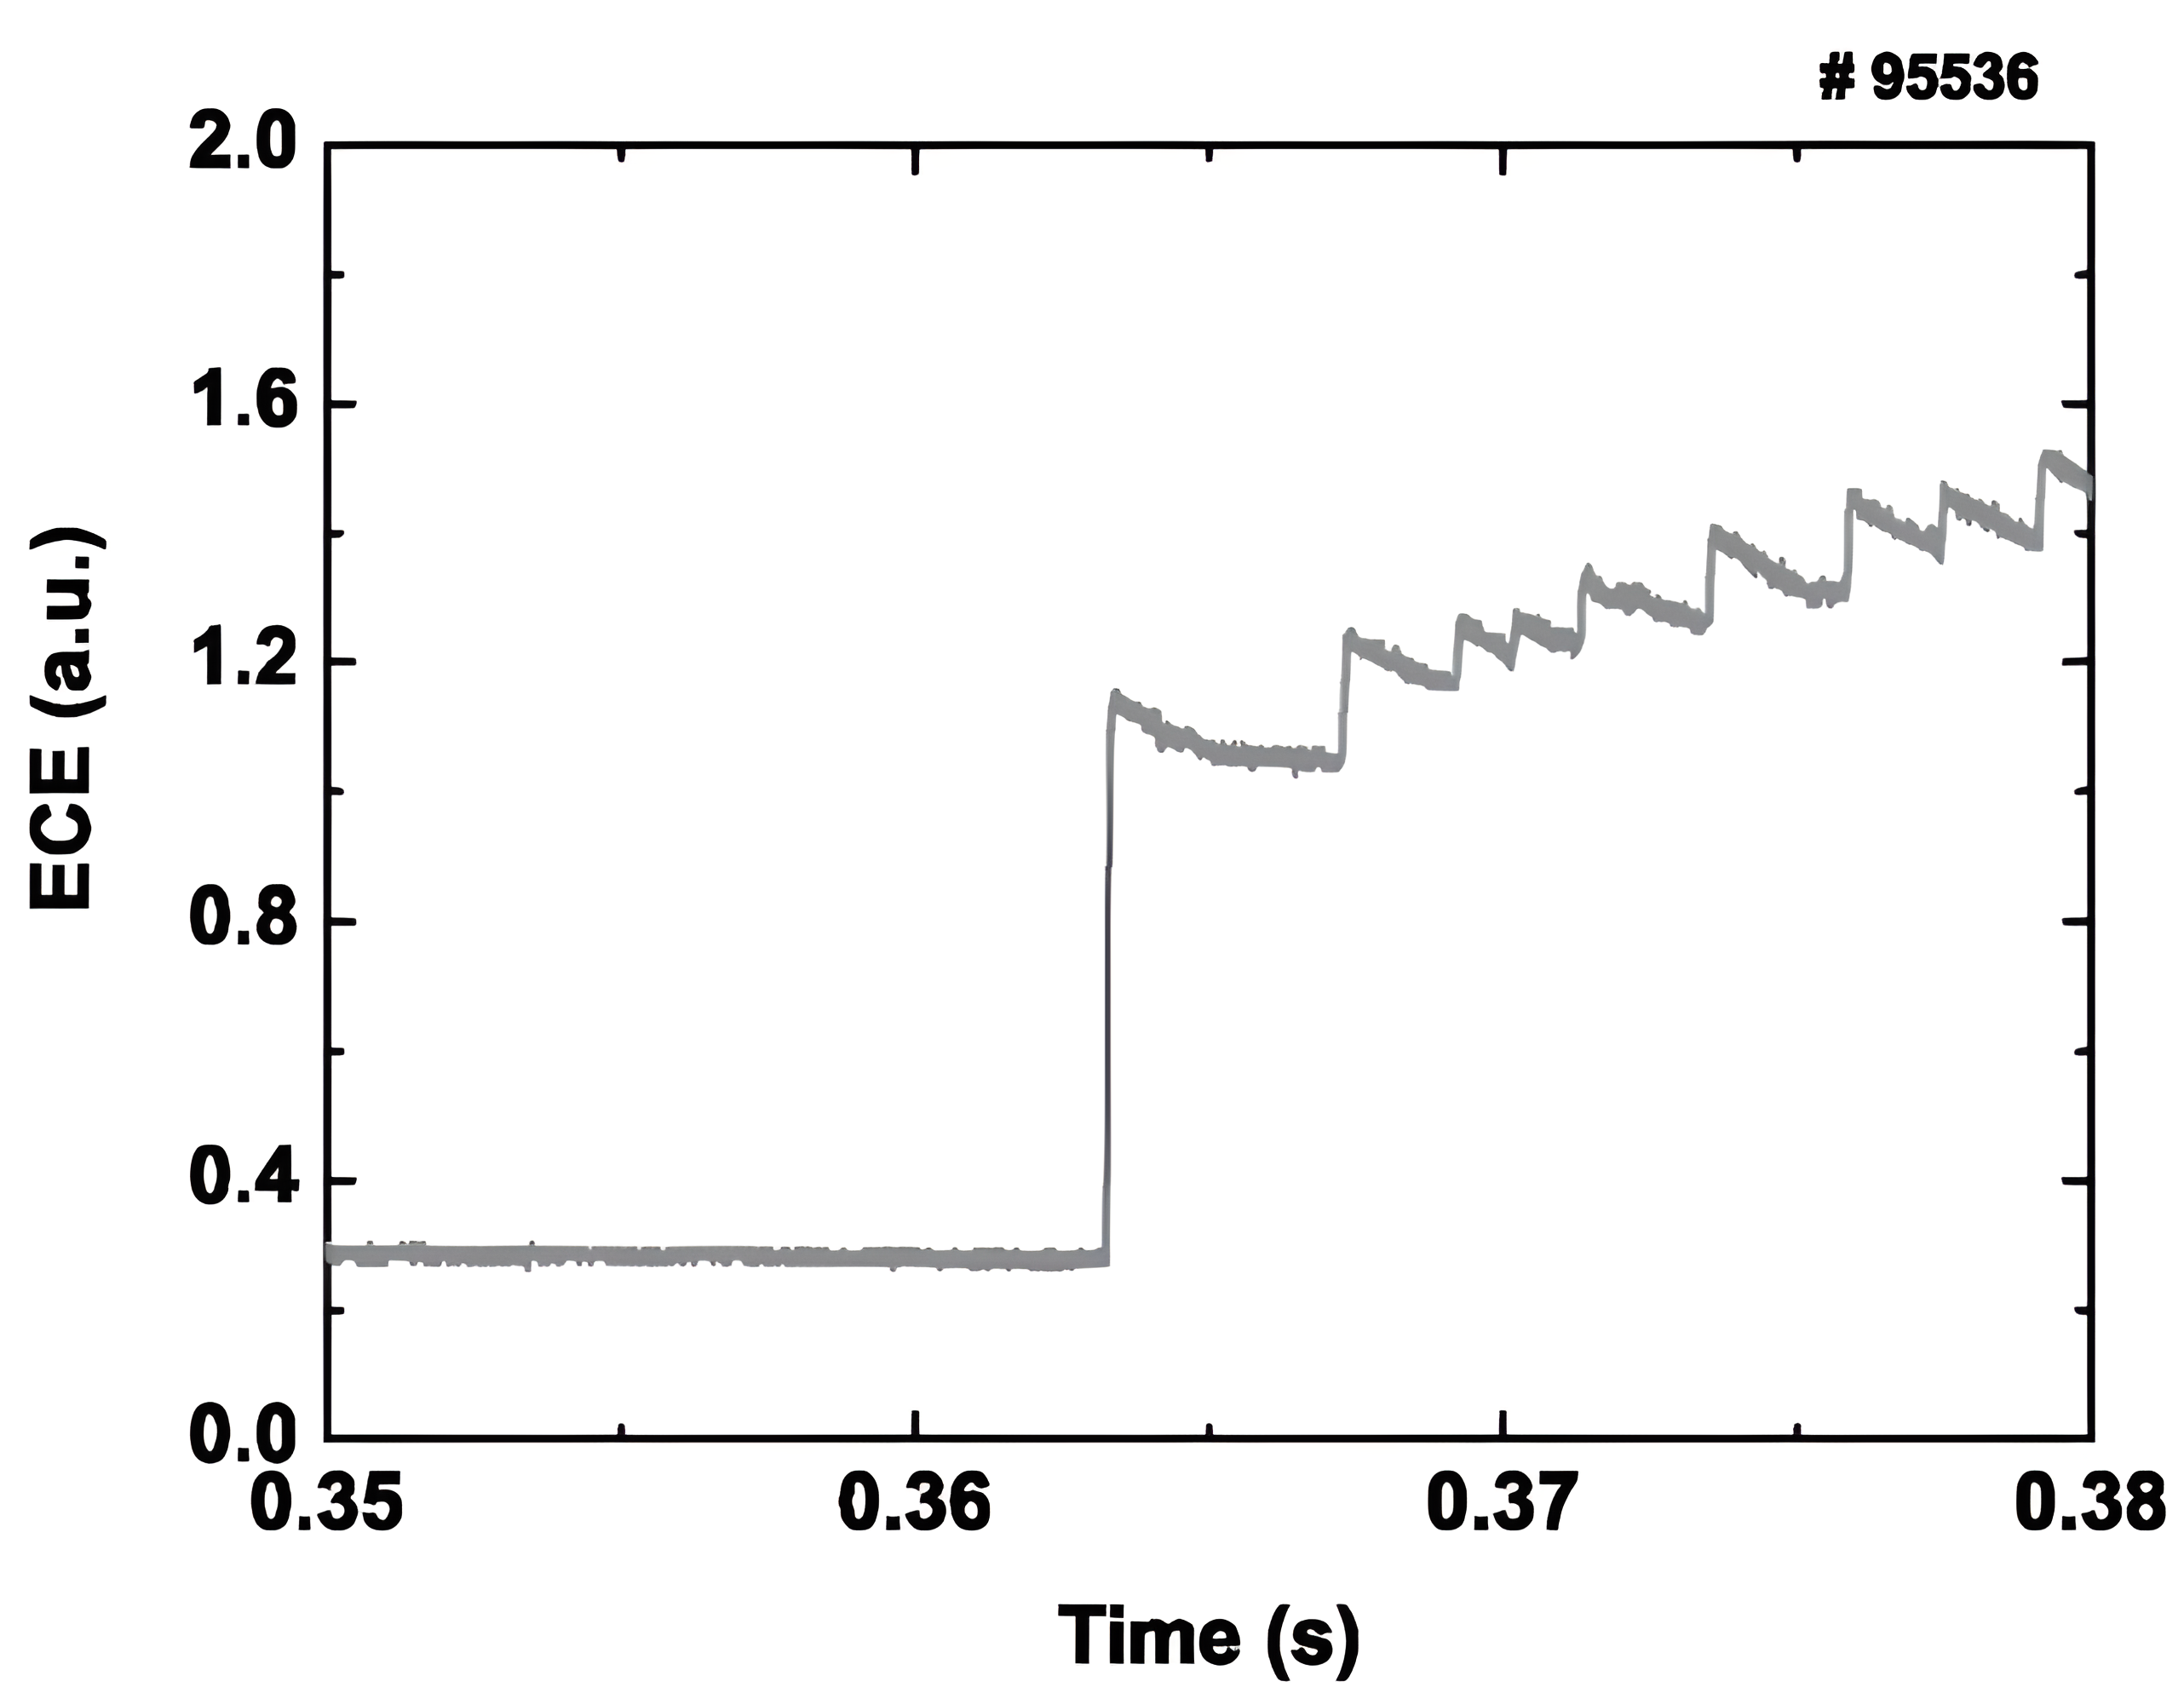
\includegraphics[width=12cm]{image27_1.png}
\caption{\label{fig:CZY1}ECE辐射中step结构\cite{RN1554},纵坐标ECE(a.u.)表示ECE测量信号强度}
\end{figure}
\begin{figure}[ht]
\centering
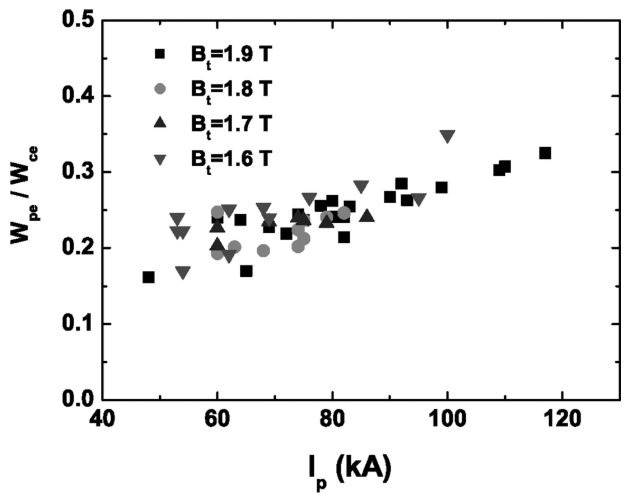
\includegraphics[width=12cm]{image28.png}
\caption{\label{fig:CZY2}不同纵场条件下不稳定性阈值和等离子体电流的依赖关系}
\end{figure}
\par 2010年,卢洪伟等人在EAST装置上研究了ECE信号step结构发生时高能电子的能量转化\cite{RN2102}。如\autoref{fig:LHW1}、\autoref{fig:LHW2}所示,在ECE出现step结构时,通过硬X 射线可以诊断不同能段逃逸电子能量迁移过程。如在$t=2.81$秒,当ECE辐射出现step跳变时(\autoref{fig:LHW1}),通过硬X射线诊断(\autoref{fig:LHW2}a)可以看出能量在1.5-2.0MeV区间逃逸电子迅速下降然后逐渐上升,而能量为9.5-10.0MeV的逃逸电子迅速上升然后缓慢下降。另一方面,\autoref{fig:LHW2}(b)FEB诊断主要用于测量电子垂直方向能量,在2.81秒ECEstep结构产生时50-100keV电子能量迅速上升,而后下降。根据以上现象,论文对该现象解释是当step结构产生时逃逸电子发生散射,其中1.5-2.0MeV逃逸电子散射到50-199keV,而更高能量的逃逸电子则散射到9.5-10.0MeV。
\begin{figure}[ht]
\centering
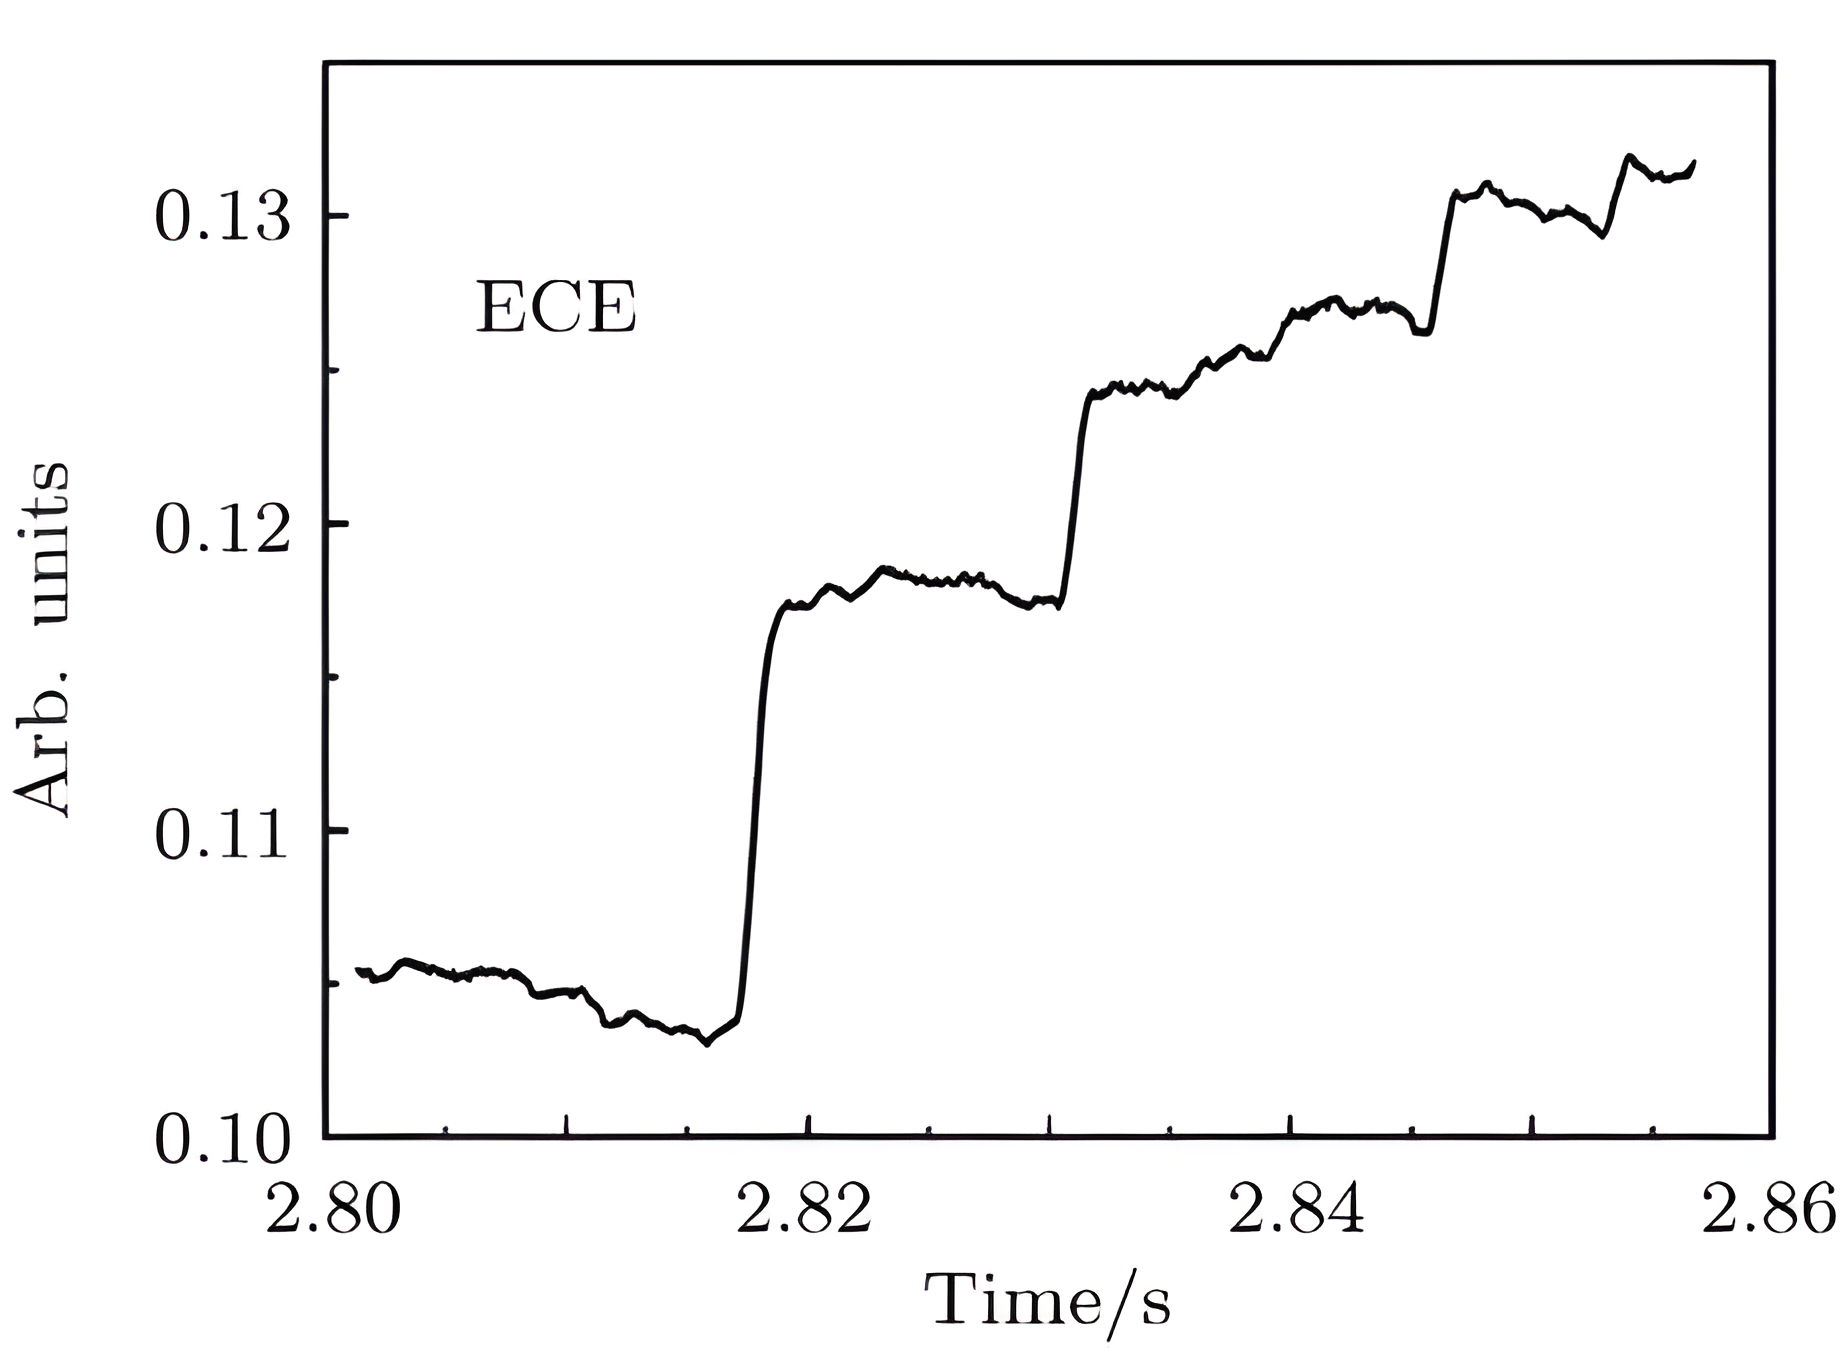
\includegraphics[width=12cm]{image29_1.png}
\caption{\label{fig:LHW1}ECE辐射细节(shot No.12964)\cite{RN2102}}
\end{figure}
\begin{figure}[ht]
\centering
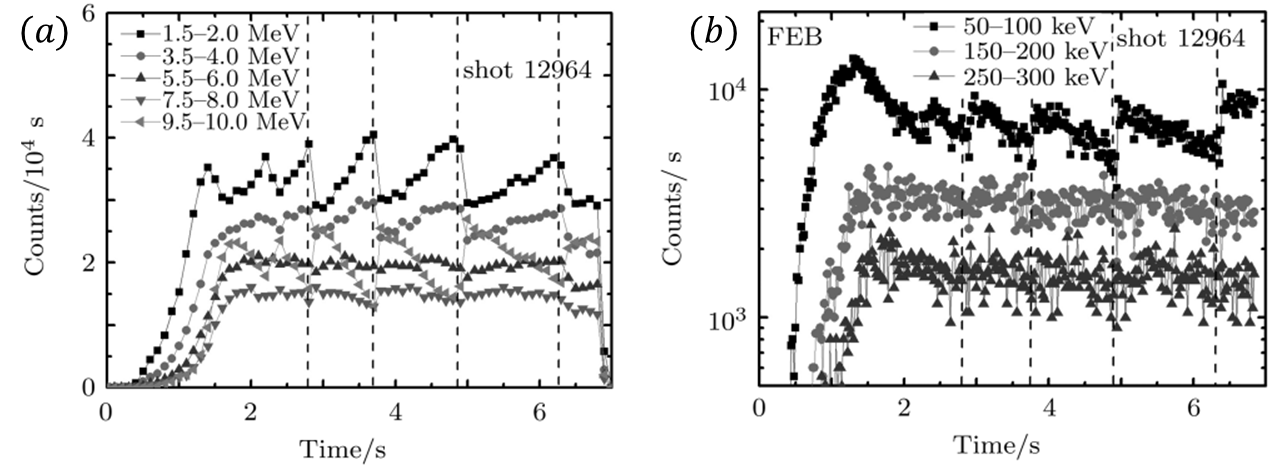
\includegraphics[width=15cm]{image30_1.png}
\caption{\label{fig:LHW2}(a)不同逃逸电子能量范围内通过硬X射线(HX)诊断检测的计数率(shot No.12964)(b)不同逃逸电子能量范围内通过快电子轫致辐射(FEB)诊断检测的计数率(shot No.12964)。图片来自Lu Hong-Wei\cite{RN2102}}
\end{figure}
\par 2015年,S. J. Freethy通过反常多普勒效应解释了在MAST装置上边界局域模(ELM)产生过程中微波辐射尖刺结构\cite{RN1868}(\autoref{fig:SGF})并且用PIC程序模拟电子速度分布函数在多普勒效应作用下随时间的演化(\autoref{fig:SGF2}),证明了反常多普勒效应会使电子速度分布函数趋向于各项同性。
\begin{figure}[ht]
\centering
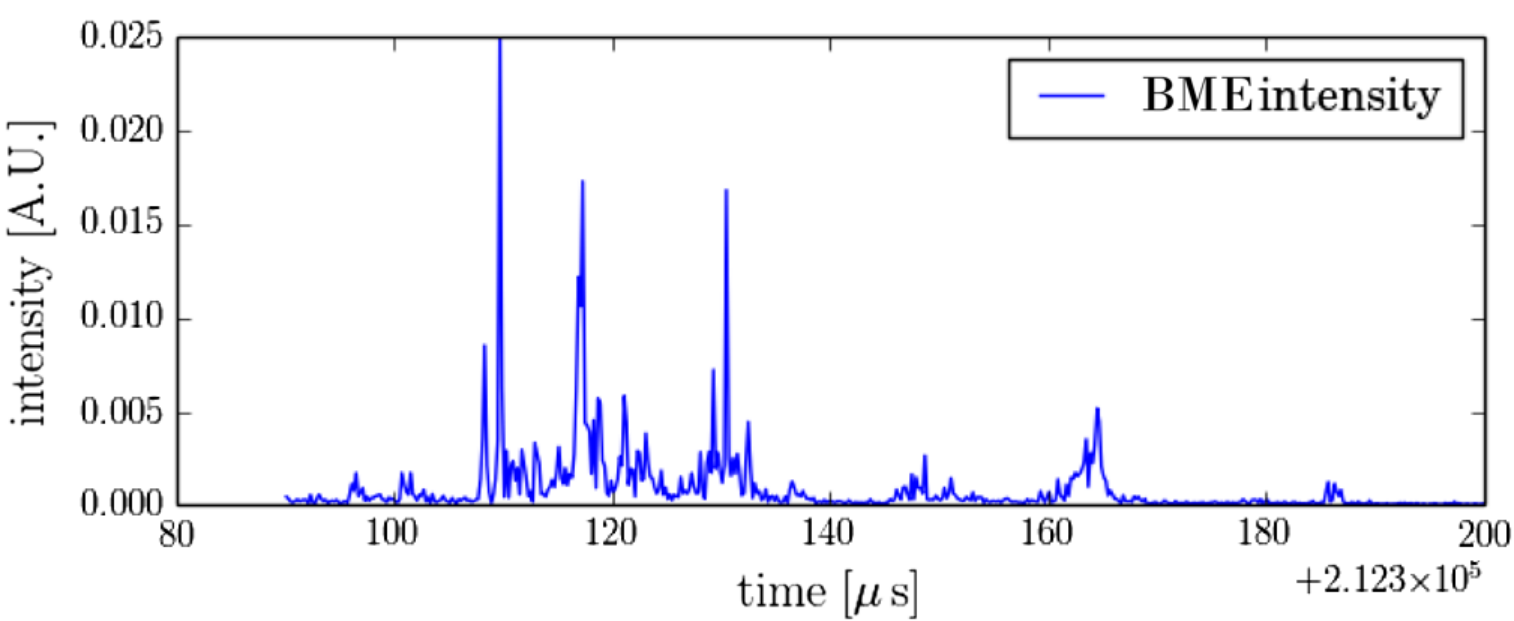
\includegraphics[width=12cm]{image31.png}
\caption{\label{fig:SGF}BMEintensity(Burst Mircowave Emission intensity)微波辐射爆发强度随时间演化\cite{RN1868}}
\end{figure}
\begin{figure}[ht]
\centering
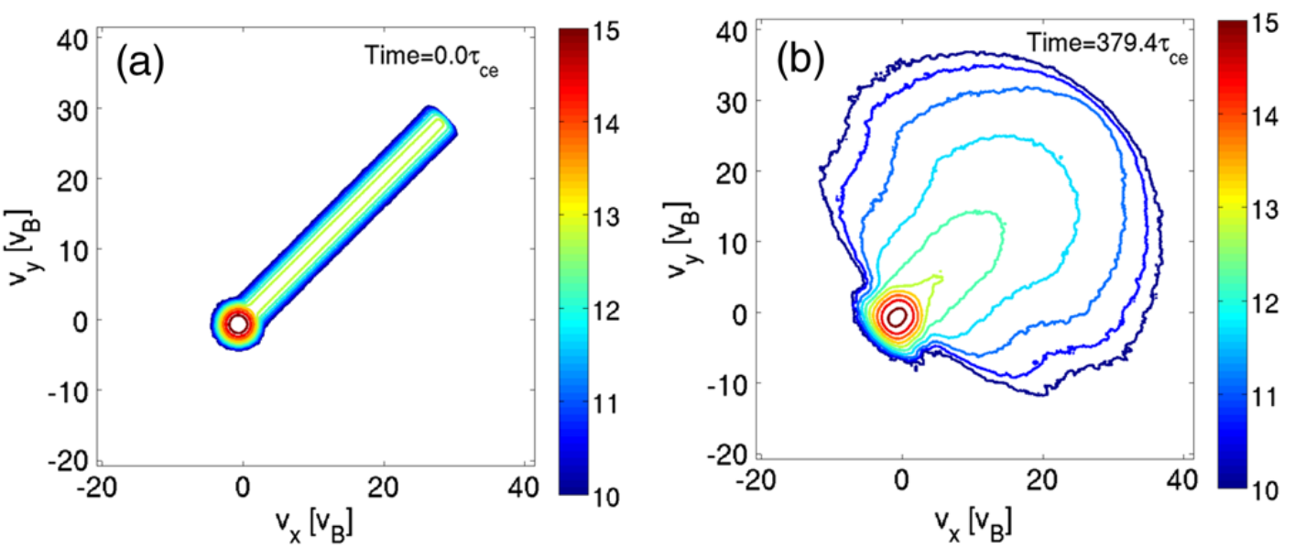
\includegraphics[width=12cm]{image32.png}
\caption{\label{fig:SGF2}PIC模拟逃逸电子分布演化(a)初始电子速度分布(b)末态电子速度分布\cite{RN1868}}
\end{figure}

\begin{figure}[ht]
\centering
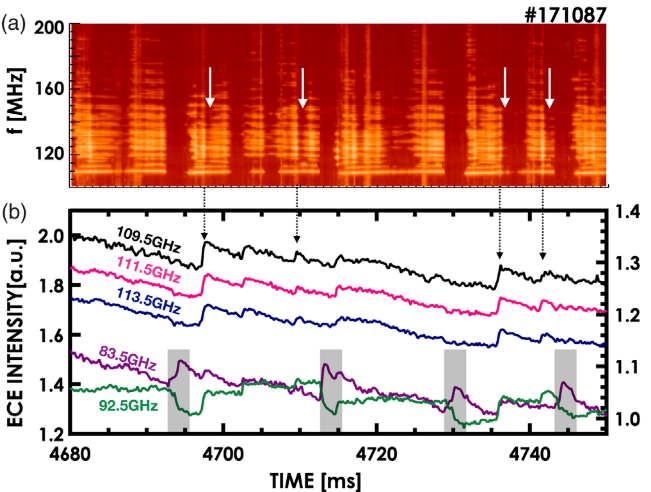
\includegraphics[width=12cm]{image33.png}
\caption{\label{fig:DAS}(a)100-200Mhz磁信号时频谱(b)不同频率的ECE信号,虚线箭头表示哨声波信号的峰值对应的ECE信号\cite{RN975}}
\note{注:图(a)中白色实线表示哨声波信号下降的时刻,图(b)中灰色区域表示n=1的锯齿活动区域}
\end{figure}

\begin{figure}[ht]
\centering
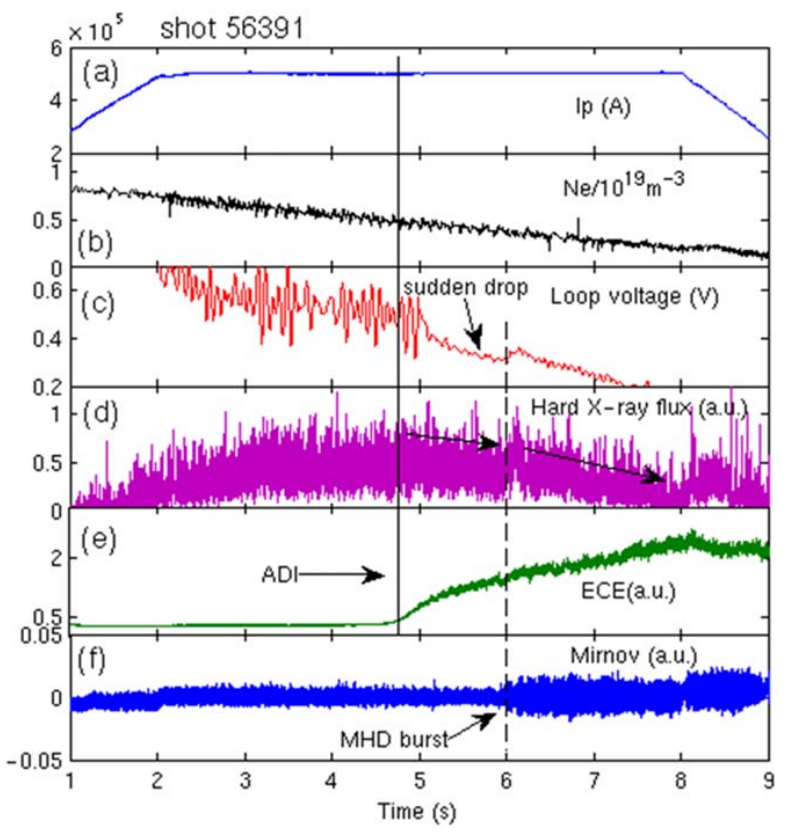
\includegraphics[width=12cm]{image34.png}
\caption{\label{fig:LEZ}EAST\#shot56391:(a)等离子体电流,(b)弦平均电子密度,(c)环电压,(d)硬X射线通量,(e)ECE辐射,(f)Mirnov 信号。垂直实线表示ECE快速爬升起点,垂直虚线表示MHD爆发时间\cite{RN1859}}
\end{figure}
\par 2018年,D. A. Spong等人在DIII-D装置首次观测到逃逸电子激发的哨声波\cite{RN975}, 如\autoref{fig:DAS}所示,其中\autoref{fig:DAS}(a)中高频磁探针测得的多支谐波频率表征高能电子激发的哨声波,\autoref{fig:DAS}(b)表示不同频率电子回旋辐射信号时序图。当哨声波强度达到峰值时,波粒相互作用导致高能电子角度散射,ECE信号迅速上升,随后哨声波强度下降。同年,刘畅利用数值模拟的方法详细分析了逃逸电子激发哨声波的过程并通过反常多普勒效应分析研究了分布函数的动理学演化\cite{RN1815}。虽然\autoref{fig:DAS}(b)电子回旋辐射形状和step结构有点相似,反常多普勒效应的研究取得了很大实验和理论上的进步,但是实际上在哨声波导致的ECE辐射信号波动和ECE的step结构在时间尺度和形状差异上还是非常明显,关于ECE辐射的step结构物理过程仍然没有得到解释。




\begin{figure}[ht]
\centering
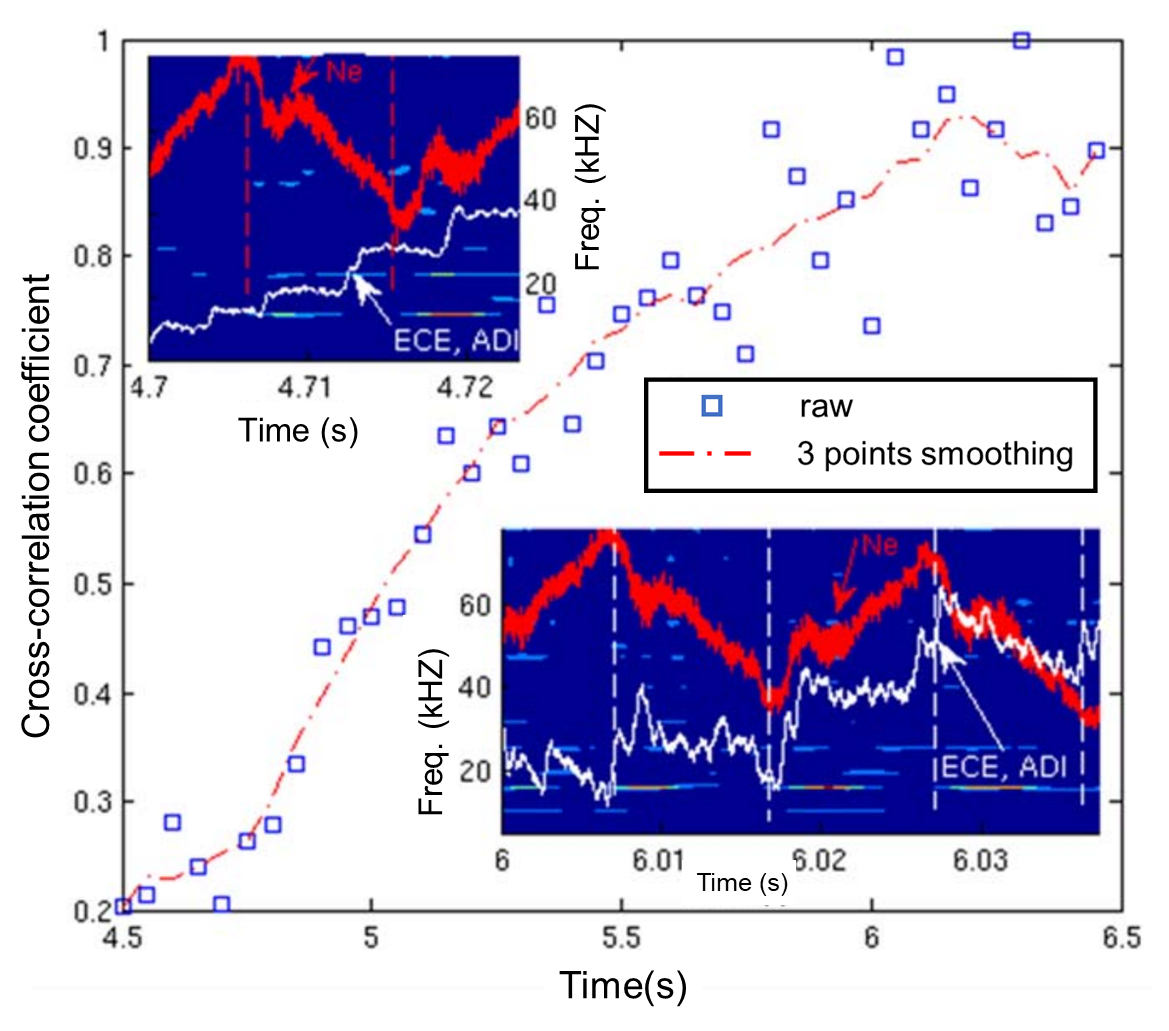
\includegraphics[width=12cm]{image35.png}
\caption{\label{fig:LEZ2}由ADI(反常多普勒不稳定性)导致的ECE信号step结构和密度波动之间的相关系数,左上图和右下图是两张不同时刻的密度波动谱并分别插入了ECE和密度时序信号\cite{RN1859}	}
\end{figure}
 \par 2020年,Li\cite{RN1859}	在EAST装置上通过线性降低等离子体密度观测到了反常多普勒不稳定性 (Anomalous Doppler Instability,ADI)。如\autoref{fig:LEZ}所示,当密度低于$0.5\times10^{19}m^{-3}$时, ECE信
号迅速升高,在4.7s和6s附近放大ECE信号可以看出ECE出现step结构
(\autoref{fig:LEZ2}),在密度波动谱中还可以看到14KHz的频谱信号。文中计算
了在[4.5s-6.5s]区间电子密度波动和ECE信号的互相关系数
\begin{figure}[ht]
\centering
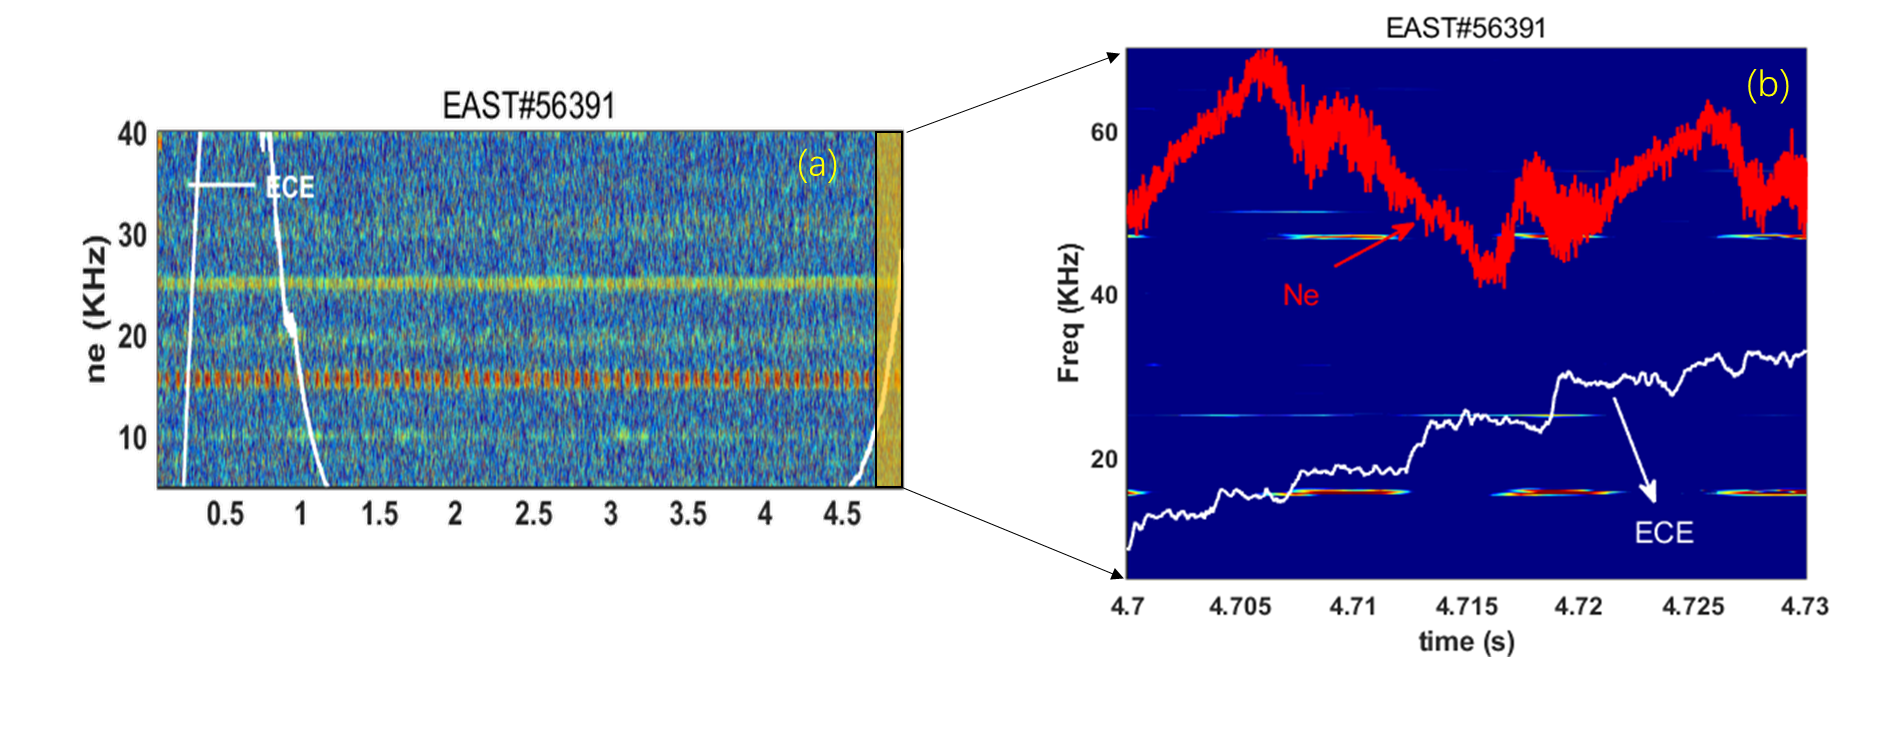
\includegraphics[width=15cm]{image36.png}
\caption{\label{fig:LEZ3}(a)放电期间密度波动谱与电子回旋辐射信号
(b)4.7s~4.73s电子回旋辐射和密度波动谱}
\end{figure}
(\autoref{fig:LEZ2})。如
\autoref{fig:LEZ2}左上角所示,$t\sim4.7s$时密度波动和ECE信号波动相关性较小,此时密度波动发生时间和ECE step上升时间不同步,而
$t\sim6s$时(如\autoref{fig:LEZ2}右下角所示,其中白色虚线
表示密度波动发生时间)密度波动和ECE信号波动具有很强的相关性,此时密度波动发生时
间和ECE step上升时间同步。磁扰动发生在$t\sim6s$之后。根据密度波动和磁扰
动频谱信号,文章指出ECE信号中ADI与磁扰动有关,但没有解释ECE step
结构上升和平台区间的形成机制。比如\autoref{fig:LEZ2}右下角所示密度频
谱(17Khz)出现的时间段内为什么ECE信号是先上升后达到平台?如何解
释\autoref{fig:LEZ2}左上角4.7s ECE step上升时间和密度波动谱出现时间不
一致的现象?这里的实验现象和论证依据还有待进一步检验。实际
上密度谱中周期性出现17KHZ谱线与磁扰动无关,更与ECE信号无关。如
\autoref{fig:LEZ3}(a)所示,这一炮中测量密度的point数据在放电全程一直存
在周期性17KHZ谱线,将其中$4.7s\sim4.73s$放大得到类似\autoref{fig:LEZ2}左上图密度谱的\autoref{fig:LEZ3}(b),所以17KHZ的谱线
是非物理的结果。而ECE信号和密度波动相关性在$t\sim6s$增大是因为出现
了MHD模,相关性增大是理所当然,和电子回旋辐射step结构似乎关系不大。




\par 2021年P Buratti 利用宽带天线在FTU装置上发现ECE辐射的step结构平台区间存在等离子体频率的辐射信号\cite{RN798}。如\autoref{fig:PBT}所示,在ECE信号step结构上升区间存在宽频的辐射爆发,而step结构平台区间存在接近等离子体频率附近的线性谱线,原因有待解释。
\par 综上所述,关于电子回旋辐射信号中出现step结构的实验报道已有很多。虽然大部分工作认为这种结构的产生与反常多普勒效应密切相关,但系统的物理分析一直欠缺。因此我们论文选择电子回旋辐射中得这一step结构开展研究,既不特殊,也不过时。显然电子回旋辐射出现 step 结构与电子速度分布函数的非热成分演化有关,这也是本论文的主要研究方向。
\begin{figure}[ht]
\centering
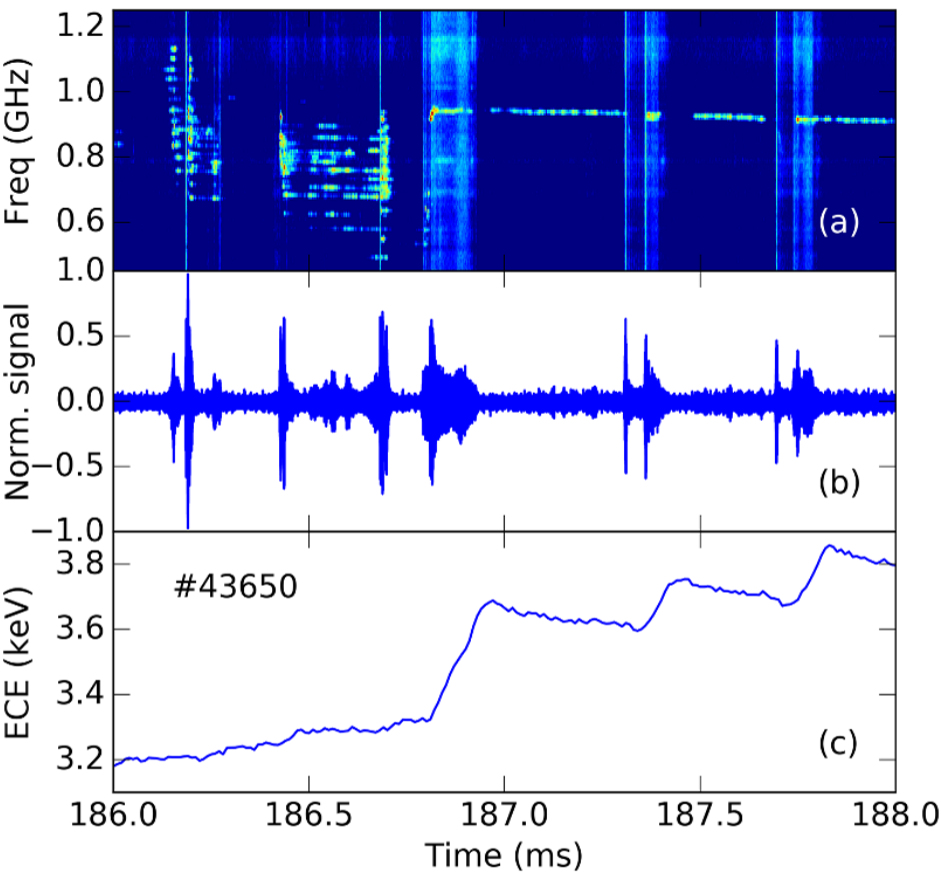
\includegraphics[width=12cm]{image37.png}
\caption{\label{fig:PBT}(a)射频辐射时频图(b)归一化射频原始信号(c)370GHz ECE辐射信号\cite{RN798}}
\end{figure}
%\clearpage
\section{研究意义}
非热化电子作为偏离热分布的一种电子速度分布状态,广泛存在与天体和实验室等离子体中。研究非热化电子产生的物理机制具有重要意义,如太阳耀斑中非热化电子与其磁重联模型之间的关系\cite{RN980},观测地球弓行激波中非热化电子有助于研究电子和哨声波的相互作用\cite{RN981},而测量地球电离层中非热化电子的能量分布又为天体中dynamo current 机制研究提供了重要指导意义\cite{RN981}。在磁约束核聚变装置放电过程中,非热化电子速度分布中的高能尾巴也会影响到磁约束等离子体中的电离、加热、输运以及磁流体稳定性。而未来的ITER装置和CFETR 等聚变堆在高参数运行下,非热化电子的影响也会更加突出\cite{RN1689}。

工欲善其事,必先利其器。电子回旋辐射成像诊断(Electron Cyclotron Emission Imaging , ECEI)是电子回旋辐射的重要诊断工具\cite{RN1020,RN1753,RN2124,RN1044,RN4},肩负着对磁流体动理学的研究任务(MagnetoHydro -Dynamics ,MHD),而且标定后的ECEI还可以测量温度分布\cite{RN1381}。ECEI数据的解读直接关系到最后的成像结果和物理分析,因此对电子回旋辐射的物理本质理解至关重要。通常等离子体需要在满足光学厚和局域热平衡条件下才能正确解读ECEI数据信号。在EAST放电初期电子密度比较低时经常出现电子回旋辐射辐射强度迅速升高,其强度约是平均热辐射强度的一个量级,该信号通常认为是由于低能非热化电子成分导致\cite{RN757}。非热化电子产生后,局域热平衡被破坏,在光学薄的条件下,ECEI信号就不能正确反映等离子体电子温度信息。这样很多时候ECEI数据就因为不满足使用条件而无法用常规方法解读。因此研究非热化电子对正确理解ECEI信号提供了指导意义。通过对ECEI信号产生的本质过程详细分析才有可能对放电过程中ECE辐射信号的各种奇特现象给出合理解释。
\par 鉴于非热化电子重要的物理性质和对电子回旋辐射的影响,各个国家也分别在不同时期开展了电子回旋辐射(ECE)辐射的相关研究。据本人所知,1958年,苏联科学家B.A.TRUBNIKOV首次提出了稀薄等离子体条件下电子回旋辐射和吸收系数的计算方法\cite{RN1003,RN1002};1961年,英国科学家BEKEFI独立提出各项同性速度分布稀薄等离子体电子回旋辐射吸收系数的计算方法\cite{RN1714}并且和1958年B.A.TRUBNIKOV得到的结果相同\cite{RN1003};1976年,C.S.Liu和Y.MOK利用单电子回旋辐射积分方法计算了逃逸电子分布函数的演化对ECE辐射的影响\cite{RN1006};1977年,H. P. Freund, and C. S. Wu提出了高密度等离子体$(ω_{ce}\sim ω_{pe})$辐射计算方法,并给出热平衡条件下各项同性麦克斯韦分布辐射谱的解析结果\cite{RN1007};1983年,M.Bronatici考虑等离子体色散效应,给出热等离子体吸收系数的计算方法\cite{RN1717};1987年荷兰R.M.J.Sillen开发ECE计算代码NOTEC\cite{RN1009};1992年,美国R.W.Harvey结合WKB射线追迹方法计算了非热化电子分布对ECE的影响\cite{RN1010};1995年,法国D.Vezard计算了少量相对论电子的电子回旋辐射和吸收系数\cite{RN2031};2008年,意大利科学家Figini编写了SPECE程序用于研究非热化电子对ECE的影响\cite{RN1013};2017年,美国普林斯顿大学的石磊博士结合M.Bornatici给出的热电子分布条件下ECE吸收系数公式,给出了热平衡条件下ECE辐射的数值合成诊断\cite{RN1014};2019年,德国SeVerin Sebastian Denk为了研究ASDEX Upgrade 托卡马克上的非热化电子编写了Erad code\cite{RN1014}。
\par 国内相关研究开展不多。1993年,丁玄同利用电子回旋辐射模型,结合极化型迈克尔逊干涉仪,分析了HL-1托卡马克中各放电阶段电子回旋辐射谱的特点\cite{RN1017}。其模型中只考虑了电子回旋辐射效应,没有考虑到电子回旋辐射在路径中的吸收效应,因此在放电初期和放电末期时,等离子体密度比较低,吸收效应不显著,模型结果和实验比较定性吻合,即一次回旋辐射强度最大,二次三次回旋频率依次减小。当放电处于密度较高的平顶段时,由于吸收效应不可忽略,辐射谱具有热辐射谱特征,因此模型得不到和实验一致的频谱。2018年中国科学院等离子体研究所ECE诊断组借助意大利SPECE程序分别研究了欧姆加热和LHW加热下ECE谱特征,并根据信号谱的形状拟合出高能尾巴的电子能量\cite{RN2115};2019年该组进一步利用SPECE程序分析了低杂波加热对ECE信号位置对应关系的影响\cite{RN1402}。

随着托卡马克放电参数不断提高, ECE诊断也会面临新的挑战。根据TFTR和JET的放电参数\cite{RN1019},当电子温度升高时,TS测量数据和ECE测量数据的偏差也会逐渐增大,这是由于电子速度在0.75$u_{th}≤u≤1.5u_{th}$区间上分布函数偏离麦氏分布。如\autoref{fig:img38}所示,导致电子在热速度附近形成非麦氏分布的原因目前还没有物理模型能够解释,除非存在很强的驱动机制,比如波粒共振打破了电子热速度分布。根据TFTR和JET观测到的参数外推ITER,当等离子体芯部温度达到20$\sim$40keV时,$T_{ECE}$和$T_{TS}$的差别将会达到50\%。所以中国发展一套数值合成诊断用于分析ECEI数据已是大势所趋。通过建立非热化电子分布和电子回旋辐射强度的关联,我们可以在非热化电子动理学演化过程中分析电子回旋辐射强度的变化。结合电子回旋辐射诊断观测到的现象,我们就可以探究实验过程中可能发生的物理过程,让我们对未来的物理诊断信号的分析具有了更加全面的认识。
\begin{figure}[ht]
\centering
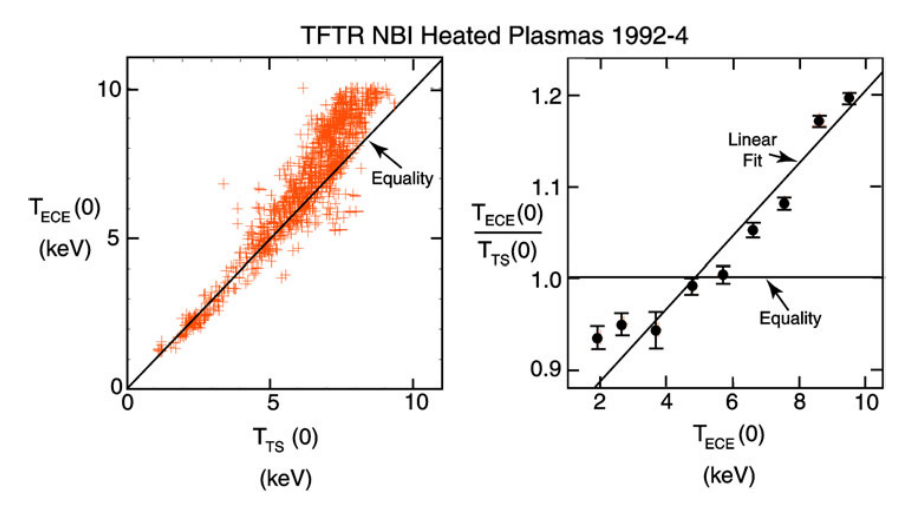
\includegraphics[width=12cm]{image38.png}
\caption{\label{fig:img38}TFTR芯部电子温度中ECE和TS测量结果,随着温度上升,测量分歧也越来越大,电子温度达到10keV时,Ts和ECE测量结果偏差达到20\%}
\end{figure}
\section{论文内容介绍}
在绪论中,本文从托卡马克放电过程入手,引出了非热化电子的产生机制,并探讨了其垂直方向温度来源与反常多普勒效应之间的联系。反常多普勒效应通常用于解释电子回旋辐射中出现的台阶状结构。然而,尽管相关研究已持续了半个多世纪,关于台阶结构的许多关键问题仍未得到解决,例如:导致电子回旋辐射出现台阶结构的具体动理学过程是什么?除了这些独特的物理现象,托卡马克放电还伴随破裂风险。当破裂发生时,会瞬间产生大量逃逸电子,其能量可达数十 MeV,这些高能电子在强电场加速下撞击第一壁或偏滤器,可能对装置造成严重损伤。然而,逃逸电子的动理学过程至今仍未完全掌握,而要避免其对装置的破坏,必须深入理解其产生机制及演化规律。

本论文的研究方法以动理学数值模拟为核心,通过求解电子速度分布的演化,计算电子回旋辐射强度与速度分布之间的关系,从而模拟不同放电条件下电子回旋辐射的演化特征。论文的章节安排如下:第二章介绍电子回旋辐射诊断系统以及观测到的反常辐射信号;第三章综述非热化电子的理论与实验研究,归纳前人的研究经验和方法,为后续的数值模拟奠定理论基础;第四章重点描述电子回旋辐射能量输运过程的计算模型,包括发射率、吸收率及传播路径等问题;第五章介绍非热化电子动理学模型的数值计算方法,并进一步研究单电子运动过程中的反常多普勒效应,详细分析其受力机理,并提出利用电磁波抑制逃逸电子的潜在方案;第六章结合实验研究非热化电子速度分布的演化,并利用动理学模型对托卡马克放电过程中观测到的电子回旋辐射变化进行深入分析。最后,第七章给出全文的总结与未来研究展望。
%
%Lorem ipsum dolor sit amet, consectetur adipiscing elit, sed do eiusmod tempor
%incididunt ut labore et dolore magna aliqua.
%\footnote{Ut enim ad minim veniam, quis nostrud exercitation ullamco laboris
%  nisi ut aliquip ex ea commodo consequat.
%  Duis aute irure dolor in reprehenderit in voluptate velit esse cillum dolore
%  eu fugiat nulla pariatur.}
